\documentclass[12pt, a4paper]{scrartcl}

\usepackage{graphicx}
\usepackage{dsfont}
\usepackage[latin1]{inputenc}
\usepackage[T1]{fontenc}
\usepackage{fancyhdr}
\usepackage{url}
\usepackage{float}
\usepackage{wrapfig}
\usepackage{tweaklist}
\pagestyle{headings}

\renewcommand{\figurename}{\footnotesize{Fig.}}
\renewcommand{\enumhook}{\setlength{\topsep}{-10pt}\setlength{\itemsep}{0pt}}
\renewcommand{\labelenumi}{(\Roman{enumi})}
\renewcommand{\labelenumii}{(\Roman{enumi}.\Roman{enumii})}
\renewcommand{\labelenumiii}{(\alph{enumiii})}
\renewcommand{\labelenumiv}{(\arabic{enumiv})}
\newcommand{\mycaption}[1]{\caption{\footnotesize{#1}}} 

\renewcommand{\topfraction}{0.9}
\renewcommand{\bottomfraction}{0.8}
\setcounter{topnumber}{2}
\setcounter{bottomnumber}{2}
\setcounter{totalnumber}{4}     
\setcounter{dbltopnumber}{2}
\renewcommand{\dbltopfraction}{0.9}
\renewcommand{\textfraction}{0.07}
\renewcommand{\floatpagefraction}{0.7}
\renewcommand{\dblfloatpagefraction}{0.7}
\addtolength{\abovecaptionskip}{-0.1in}
\addtolength{\belowcaptionskip}{-0.1in}

\author{Clemens Lode}

\begin{document}

\thispagestyle{empty}
\noindent
\begin{tabular}{ll}
  \hspace{-2mm}
  \parbox[b]{0.88\textwidth}
  {
    \flushleft
    Institut f�r Angewandte Informatik\\
    und Formale Beschreibungsverfahren\\
    Universit�t Karlsruhe (TH)\\
    \vspace{1em}

    Forschungsgruppe Effiziente Algorithmen\\
    Prof. Dr. Hartmut Schmeck\\
  } & 
\includegraphics[height=7em]{AIFB_Logo_senkrecht.png}\\

\end{tabular}

\vspace{2cm}
\begin{center}{\bf \LARGE Studienarbeit}\\
\vspace{2cm}
{\bf "Reducing diversity loss in estimation of distribution algorithms"}\\
\vspace{1cm}
von
\vspace{1cm}
{\bf Clemens Lode}\\
\vspace{1cm}
eingereicht am 15.11.2006\\
beim Institut f\"ur Angewandte Informatik\\
und Formale Beschreibungsverfahren (AIFB)\\
der Universit\"at Karlsruhe (TH)\\
\vspace{2cm}
Betreuer:	&J\"urgen Branke\\
Referent:	&Prof. Dr. H. Schmeck\\
\vspace{2cm}
\begin{tabbing}
xxxxxxxxxxxxxxxx\=xxxxxxxxxxxxxxxx\kill
Heimatanschrift:\>Studienanschrift:\\
Edelwei\"sweg 16\>L\"otzener Stra\"se 16\\
87493 Lauben\>76139 Karlsruhe\\
clemens@lode.de\\
\end{tabbing}

\end{center}

%\noindent
%Studienarbeit "Reducing diversity loss in estimation of distribution algorithms"\\
%Sommersemester 2006
%\vspace{3cm}

%\noindent
%{\Large\textbf{Reducing diversity loss\\ in estimation of distribution algorithms}}

%\vspace{3cm}

%\noindent
%\begin{tabular}{ll}
%Autor:	  &Clemens Lode\\
%Betreuer:	&J\"urgen Branke
%\end{tabular}

\newpage

\tableofcontents

\newpage

\section{Introduction}

Many Estimation of Distribution Algorithms (EDAs) can reach a state where the probability of ever finding the optimum is zero. This is due to diversity loss, i.e. one or more components of all individuals in the populations become the same value. If a different value is required for the optimal solution, the optimum will never be sampled. If no action is taken to either prevent uniformity of the values in a single component or to reduce the diversity loss in each generation, the variance can never be restored or held at a certain level and simply increasing the number of generations will not increase the probability of finding the optimal or even a better solution.\\
One way to counter this diversity loss is to increase the population size, by checking and correcting the populaton if uniformity in a component is reached or by using the Laplace correction. This report will use a different approach by adjusting the distribution vector according to the population size, selection size and generation method. Several methods will be compared and 

\section{Abstract}

In \cite{Shapiro} it was shown that the expected factor of diversity loss of sampling \(N\) individuals from a population of the size \(M\) and generating a new population of the size \(M\) is \(1 - \frac{1}{N}\) and that this is true for a whole class of EDAs (SML-EDAs, probability model is build using only data sampled from the last generation). In this report it will be shown that the factor of diversity loss of randomly generating a new population of the size \(M\) on the basis of a distribution vector \(p\) is \(1 - \frac{1}{M}\). Using both results we can calculate a new \(p\) (on the basis of the population size \(M\), the sampling size \(N\) and the old distribution vector) with which the diversity loss is lower. The diversity loss can be reverted with the factor \(x = \frac{N(M-1)}{M(N-1)}\). This method, which will be called {\bf Random Distribution Correction} (RDC), outperforms the standard Laplace correction in problems like OneMax. In addition it will be shown that, instead of randomly creating a new generation by applying the distribution vector \(p\) on each single component of all individuals of the population, distributing exactly \(p \cdot M\) '1's in the population will result in a total loss of diversity of only \(\frac{M(N-1)}{N(M-1)}\) instead of \(1 - \frac{1}{N}\) and that this loss can be corrected in the same manner as with RDC. This method will be called {\bf Exact Distribution Correction} (EDC) and significantly outperforms RDC at the cost of a lower convergence speed. The resulting method corrects \(p\) to \(\frac{1}{2}(1 - \sqrt{1 - x)}\) for \(p < \frac{1}{2}(1 - \sqrt{1 - \frac{1}{x}})\), to \(\frac{1}{2}(1 + \sqrt{1 - x})\) for \(p > \frac{1}{2}(1 + \sqrt{1 - \frac{1}{x}})\) and to \(\frac{1}{2}\) otherwise.\\

\newpage
\section{Definitions}

The diversity of a given population can be measured by the trace of the empirical co-variance matrix.\\ TODO
Let
\begin{itemize}
\addtolength{\itemsep}{-0.5\baselineskip}
\item \(C\): number of components of each individual
\item \(N\): size of the population
\item \(n\): number of selected individuals
\item \(A\): set of different values a component can take
\item \(|A|\): number of different values a component can take
\item \(x^{\mu}_{i}\): value of component i of individual \(\mu\)
\item \(\varphi(x)\): '1' if the condition x is met, '0' otherwise
\end{itemize}

\subsection{Variance of a population}

\(v^{a}_{i}\) describes the ratio of a certain value of a component in the population. E.g. \(v^{0}_2 = 0.3\) means that 30\% of all the individuals in the population have a '0' in the second component. 
\begin{equation}
\label{eq:variance1}
v^{a}_{i} = \frac{1}{N} \sum_{\mu=1}^{N} \varphi(x^{\mu}_{i} = a)
\end{equation}

\(v_{i}\) denotes the average variance of all values of a certain value of a component in the population.
\begin{equation}
\label{eq:variance2}
v_{i} = \frac{1}{|A|} \sum_{a=0}^{|A|-1} v^{a}_{i} (1 - v^{a}_{i})
\end{equation}

\(v\) denotes the sum of the average variances of all values of the values in all components in the population.
\begin{equation}
\label{eq:variance3}
v = \frac{1}{|A|} \sum_{i=1}^{C} \sum_{a=0}^{|A|-1} v^{a}_{i} (1 - v^{a}_{i})
\end{equation}

The scope of this report is to apply Univariate Marginal Distribution Algorithms ({\bf UMDA}s) on problems with a flat fitness landscape. UMDAs assume independence between variables, i.e. we examine each component independently and set \(C = 1\). TODO

TODO evtl neuformulieren
Although there are implementations of UMDA with \(|A| > 2\) (see \cite{Unknown1}) we will only look into the case of \(|A| = 2\), i.e. our UMDAs are represented as bit-strings.\\

As defined above, \(v\) denotes the sum of the average variances of all values of all components in the population. With \(|A| = 2\) and with \(k = (k_{1}, k_{2}, ..., k_{C})\), with \(k_{i}\) denoting the number of '1's in the \(i\)th component, we get for equation~\ref{eq:variance3}:
\[
v = \frac{1}{2} \sum_{i=1}^{C} \sum_{a=0}^{1} v^{a}_i (1 - v^{a}_i)
\]
and for a given \(k\) we can calculate the \(v^{a}_i\)'s 
\[
v^{a=0}_{i} = \frac{M - k_{i}}{M}
\]
\[
v^{a=1}_{i} = \frac{k_{i}}{M}
\]
This is true because \(\sum_{\mu=1}^{M} \varphi(x^{\mu}_i = 1) = k_{i}\) and \(\sum_{\mu=1}^{M} \varphi(x^{\mu}_i = 0) = (M - k_{i})\).\\

So we get:

\[
v = \frac{1}{2} \sum_{i=1}^{C} \sum_{a=0}^{1} v^{a}_i (1 - v^{a}_i) = \frac{1}{2} \sum_{i=1}^{C} [v^{0}_i (1-v^{0}_i) + v^{1}_i (1 - v^{1}_i)] =
\]
\[
      \frac{1}{2} \sum_{i=1}^{C} [\frac{M - k_i}{M} (1 - \frac{M-k_i}{M}) + \frac{k_i}{M} (1 - \frac{k_i}{M})] = {\bf \sum_{i=1}^C \frac{k_i M - k^{2}_{i}}{M^{2}}}
\]
And
\begin{equation}
\label{eq:variance4}
	v_{i} = \frac{k_i M - k^{2}_{i}}{M^{2}}
\end{equation}

\subsection{Random Distribution with UMDAs (RD)}

With UMDAs we determine in each step the ratio of '1' for each component of the selected part of the population and calculate the ratio. In the literature (see \cite{Muehlenbein}) this is usually called \(p_{i}\) and it is equal to our definition of \(v^{a=1}_{i}\), so we set \(p_{i} := v^{1}_{i}\). The distribution vector is called \(p := {p_{1}, p_{2}, ..., p_{C}}\).\\
From this distribution vector \(p\) a new population of the size \(M\) is generated where each individual has a '1' in its \(i\)th component with the probability \(p_{i}\) (or likewise a '0' with the probability \((1 - p_{i})\)). The distribution vector of the next generation will be called \(p_{t+1}\) and this way of creating a new generation will be called {\bf Random Distribution} (RD). In chapter 5 we will look into a different method, called Exact Distribution (EC), which distributes exactly \(p \cdot M\) '1's within the population. If no correction method (correction methods will be discussed later) is applied, it will simply be called {\bf No Correction} (NoC).\\

The probability for \(p_{t+1;i} = \frac{k_{i}}{M}\), i.e. the probability for generating a population with \(k_{i}\) '1's in the \(i\)th component on the basis of a given distribution vector \(p\), is
\begin{equation}
\label{eq:probabilityk}
P(p_{t+1;i} = \frac{k_{i}}{M}) = p^{k_{i}}_{t;i} (1 - p_{t;i})^{M - k_{i}} {M \choose k_{i}}
\end{equation}

\subsection{Expected Variance of a population}
We have on the one side the probability for the generation of a population with a certain \(k\) and a given \(p\) (equation~\ref{eq:probabilityk}) and the variance of such a population (equation~\ref{eq:variance4}). The expected variance \(d_p\) of the whole population on the basis of \(p\) and \(M\) is therefore the sum over all products of the variance and the probability of all values of \(k_{i}\):
\begin{equation}
\label{eq:totalv}
d_p = \sum_{i=1}^C \sum_{k_{i}=0}^{M} v_{k_{i}} P(p_{t+1;i} = \frac{k_{i}}{M}) = 
\sum_{i=1}^C \sum_{k_{i}=0}^{M} \frac{k_i M - k^{2}_{i}}{M^{2}} p^{k_{i}}_{i} (1 - p_{i})^{M - k_{i}} {M \choose k_{i}}
\end{equation}

\newpage
\section{Preventing variance loss with Random Distribution Correction (RDC)}

We will now examine a single component and how to prevent some of the variance loss that happens from one generation to the next. As previously stated in the scope of this report (UMDAs) each component is independent, i.e. \(C = 1\) and we set \(k = k_{i=1}\) and \(p = p_{i=1}\) for simplicity. The creation of one generation is as follows:

\begin{figure}[H]
\setbox0\vbox{\small
Given: Population of the previous generation $\Rightarrow$Variance \(v_{t}\)\\
\begin{enumerate}
\item Select \(N\) individuals and calculate \(p\)\\
\item Generate new population of size \(M\) on basis of \(p\) $\Rightarrow$Variance \(v_{t+1}\)\\
\end{enumerate}
}
\centerline{\fbox{\box0}}
\end{figure}

\subsection{Variance loss}

From \cite{Shapiro} we know that the variance loss of the two steps on a flat landscape with Random Distribution is \(1 - \frac{1}{N}\), i.e. (with \(v_{t}\) denoting the variance of the population of the last generation from which we have selected \(N\) individuals and \(v_{t+1}\) denoting the variance of the current population)

\begin{equation}
v_{t+1} = (1-\frac{1}{N})v_{t}
\end{equation}

When generating a new population on basis of \(p\) we learned last chapter (equation~\ref{eq:totalv}) that the total variance of the population that we will have after step (II) is \(d_{p}\). But the variance that we want is \(p ( 1 - p )\), i.e. the variance of a population of infinite size generated on basis of \(p\) and no variance loss. So the factor of variance loss of step (II) is \(\frac{d_p}{p(1-p)}\). Using for example the math program Maple this can be simplified to:
\begin{equation}
\label{eq:dcorrection}
\frac{d_p}{p(1-p)} = \frac{1}{p(1-p)} \sum_{k=0}^{M} \frac{k M - k^{2}}{M^{2}} p^{k} (1-p)^{M - k} {M \choose k} = {\bf 1 - \frac{1}{M}}
\end{equation}

So we have:
\begin{itemize}
\addtolength{\itemsep}{-0.5\baselineskip}
\item Factor of variance loss of step (II) : \(1 - \frac{1}{M}\) (from (\ref{eq:dcorrection})\\
\item Factor of Variance loss of step (I) and (II) together : \(1 - \frac{1}{N}\) (from \cite{Shapiro})\\
\end{itemize}

Our factor \(y\) of variance loss of step (I) is therefor: 
\begin{equation}
\label{eq:y}
1 - \frac{1}{N} = y \frac{d_p}{p(1-p)} \Leftrightarrow y = \frac{1 - \frac{1}{N}}{\frac{d_p}{p(1-p)}}
\end{equation}

With equation~(\ref{eq:dcorrection}) we get \(y = \frac{1 - \frac{1}{N}}{1 - \frac{1}{M}} = \frac{M(N-1)}{N(M-1)}\).\\

\subsection{Distribution vector correction}

% TODO vielleicht noch einschraenkend sagen, dass man nur den Varianzverlust von Schritt III reparieren kann 
%We cannot correct the diversity loss that is happening in step (II) by changing

If we use a different distribution vector \(q\) to generate the population and set \(q(1-q)\) (or \(q\) accordingly) in a way so that the theoretical factor of variance loss is 1 (i.e. no variance loss) we will reduce the overall variance loss. For now we will try to reduce the variance loss of only step (I), the variance loss of step (II) will be discussed in chapter 5.\\
As our variance loss in step (I) is \(y = \frac{M(N-1)}{N(M-1)}\) we have to multiply with the reciprocal value in order to nullify the variance loss and multiply that factor with our original \(p(1-p)\) variance. We are allowed to do that because the variance loss itself does not depend on the distribution vector we use:

\begin{equation}
x = \frac{1}{y} = \frac{N(M-1)}{M(N-1)}
\end{equation}

\begin{equation}
\label{eq:qpx}
q(1-q) = p(1-p) x \Leftrightarrow -q^2 + q - (-p^2 + p) x = 0 \Leftrightarrow q_{1/2} = \frac{1}{2} (1 \pm \sqrt{1 - 4 (-p^2 + p) x})
\end{equation}

For \(1 - 4 (-p^2 + p) \frac{N(M-1)}{M(N-1)} < 0\) we get a negative value in square root. The border values for p are:
\[
1 - 4 (-p^2 + p) \frac{N(M-1)}{M(N-1)} = 0 \Leftrightarrow
\]
\[
p_{1/2} = \frac{1}{2} (1 \pm \sqrt{1 - \frac{M(N-1)}{N(M-1)}})
\]
\\
\begin{wrapfigure}{r}[0cm]{5.5cm}
\includegraphics[scale=0.4]{graphs/graph_correction/graph_random_distribution_correction.png}
\mycaption{Correction graph for Distribution Correction}
\label{dc_correction_1}
\end{wrapfigure}

If our \(p\) is within \(p_{1}\) and \(p_{2}\)
\[
\frac{1}{2} (1 - \sqrt{1 - \frac{M(N-1)}{N(M-1)}}) < p < \frac{1}{2} (1 + \sqrt{1 - \frac{M(N-1)}{N(M-1)}})
\]
we will have to substitute with an appropriate value. As the function approaches \(0.5\) both from the top and from the bottom we will substitute with \(q = 0.5\) if our \(p\) is within those borders. In Figure \ref{dc_correction_1} you can see the graph of the correction function for a population size of 10. The green line represents \(f(p) = p\), i.e. no correction takes place. The larger the population size is the smaller is the horizontal line in the middle, i.e. the substitution with \(p = 0.5\).

\subsection{Code}
Finally we can put our results into a code, \(M\) is our population size \(N\) is our sampling size:\\
         
\begin{verbatim}
if( p < (1 - sqrt( 1 - (M*(N-1)) / (N*(M-1)) ) )/2 )
    q = (1 - sqrt( 1 - (N*(M-1)) / (M*(N-1)) * 4*p*(1-p) ) )/2;
else 
if( p > (1 + sqrt( 1 - (M*(N-1)) / (N*(M-1)) ) )/2 )
    q = (1 + sqrt( 1 - (N*(M-1)) / (M*(N-1)) * 4*p*(1-p) ) )/2;
else
    q = 1/2;
\end{verbatim}

It is easy to implement the code piece within an existing application as it is problem independent (within the restrictions described above, bit-strings on a flat landscape in UMDA). The code itself has to be inserted just after determining the distribution \(p\) from the selected part of the population of the size \(N\) and before generating the new population.

\newpage
\section{Exact Distribution (ED)}

So far we have calculated that the variance loss of generating a population on basis of \(p\) randomly (i.e. with RD) in step (II) will result in a variance loss of \(1 - \frac{1}{M}\) (equation~\ref{eq:dcorrection}). In order to create a new generation we originally set each value of each component of an individual of the new population to '1' with the probability of \(p\) (or to '0' with the probability of \(1-p\)). \\
We can further reduce the variance loss if we create the new generation by distributing exactly \(p \cdot M\) '1's (or \((1-p) M\) '0's) within the array of components in the population so that the new variance is exactly \(p (1 - p)\), i.e. there will be no variance loss in step (II). You can see that in Figure \ref{exact_distribution_1}, the methods using ED perform better in fitness and in diversity. You can also see that it has a lower convergence rate with simple problems like OneMax which is because with Random Distribution the population can change faster.
TODO evtl runter
For this method our \(p\) is calculated this way:
\[
p = \frac{k_{old}}{N} \quad \mbox{and} \quad
k_{new} = \lfloor p M \rfloor = \left \lfloor \frac{k_{old} M}{N} \right \rfloor
\]

\(k_{old}\) denotes the number of '1's in the last generation, \(k_{new}\) denotes the number of '1's in the generation we are about to create. \(\lfloor p M \rfloor = \lfloor \frac{k_{old} M}{N} \rfloor\) does only apply when we do not change \(p\) through any correction method (like Laplace Correction).\\


\begin{figure}[H]
\hspace{-0.5in}
\includegraphics[scale=0.5]{graphs/graph_flat1163174282/graph_flat000_diversity.png}
\includegraphics[scale=0.5]{graphs/graph_onemax1163174291/graph_onemax000_fitness.png}
\mycaption{Comparison between Exact Distribution and Random Distribution}
\label{exact_distribution_1}
\end{figure}

\subsection{Exact Distribution Correction (EDC)}

When using an Exact Distribution the diversity loss in step (II) is expected to be different compared to the diversity loss of Random Distribution (\(1 - \frac{1}{M}\)). For now we will ignore the rounding error and assume that there are exactly \(p \cdot M\) '1's in the population. We have to change in equation~(\ref{eq:probabilityk}) the probability for \(\tilde{p_{i}} = \frac{k_{i}}{M}\) accordingly:

\[
\dot{P_(\tilde{p_{i}}} = \frac{k_{i}}{M}) = \left\{
\begin{array}{l l}
1 & \quad \mbox{for \(k_{i} = p_{i}M\)}\\
0 & \quad \mbox{for \(k_{i} \neq p_{i}M\)}\\
\end{array}
\right.
\]

The other equations (\ref{eq:variance1}), (\ref{eq:variance2}), (\ref{eq:variance3}), (\ref{eq:variance4}) about our variance \(v_{i}\) remain the same as they are dependent on our \(k_{i}\) anyways. Changes have to be made to equation~(\ref{eq:totalv}) because our \(P(\tilde{p_{i}} = \frac{k_{i}}{M})\) has changed. We no longer sum over all possible values of \(k\) as only (\(k = p \cdot M\)) has the probability '1' while all other values for \(k\) have the probability '0':

\begin{equation}
\dot{d}_p = \sum_{i=1}^C  v_{k_{i} = p_{i} M} P(\tilde{p_{i}} = \frac{k_{i} = p_{i}M}{M}) = 
\sum_{i=1}^C \frac{p_{i} M^{2} - (p_{i} M)^{2}}{M^{2}} = 
\sum_{i=1}^C p_{i} (1 - p_{i})
\end{equation}

As expected we have no loss of variance in step (II) using Exact Distribution because \(\frac{\dot{d}_p}{p(1-p)} = 1\). From chapter 4 we know that the expected variance loss in step (I)  is \(\frac{M(N-1)}{N(M-1)}\) (equation~\ref{eq:y}) which is now also our expected total variance loss from step (I) and (II) together. Using same the correction method from chapter 4 our expected variance loss should therefor be zero instead of \(1 - \frac{1}{M}\) as with the Random Distribution.
In Figure \ref{comparison_exact_1} you can see that compared with RDC from the previous chapter 'Exact Distribution Correction' has the lowest variance loss on a flat fitness landscape.
TODO fitness

\begin{figure}[H]
\hspace{-0.5in}
\includegraphics[scale=0.5]{graphs/graph_flat1163174262/graph_flat000_diversity.png}
\includegraphics[scale=0.5]{graphs/graph_onemax1163174272/graph_onemax000_fitness.png}
\mycaption{Exact Distribution Correction has the lowest variance loss and reaches the highest fitness level}
\label{comparison_exact_1}
\end{figure}

\newpage
\subsection{Rounding errors}

The problem is that we actually cannot use the new distribution vector that we calcuated with EDC to generate the new population because we have demanded that \(p \cdot M\) is an integer.\\
When we simply calculate \(p\) by counting the number of '1's in the selected part of the population of size \(N\) such a rounding error will only occur if \(M\) is no multiple of \(N\). But if we change the distribution vector then our new \(p \cdot M\) will probably be no integer and we would have to change our EDC algorithm. So we have a mutual dependency between our algorithm and \(p\).\\
Thus, when using Exact Distribution, we either solve that dependency which is difficult to accomplish (see chapter 5.3). Or we ignore the error in our algorithm and either round to the nearest integer or, depending on the remainder, randomly decide whether to add another '1' (e.g. for \(p = 0.71\) and \(M = 10\) we would distribute seven '1's and an eighth '1' with the probability of \(0.1\)).\\
The drawback for the latter two methods is that the distribution no longer deserves the title 'exact' because we ignore the error from the ignored dependency although we still get a lower variance loss as seen in the tests. We will take a short look into the first method in the next section.
TODO evtl raus

\subsection{Real Exact Distribution Correction}

As discussed in the previous section we cannot demand that our \(p \cdot M\) is an integer while changing the \(p\) with EDC as discussed earlier. Using the second method mentioned in the Rounding Errors section (randomly decide whether to generate one additional '1') in equation~(\ref{eq:probabilityk}) the probability for \(\tilde{p_{i}} = \frac{k_{i}}{M}\) obviously changes as there are \(\lfloor p \cdot M \rfloor\) '1's with the probability \(1-(p \cdot M - \lfloor p \cdot M \rfloor)\) and \(\lfloor p \cdot M \rfloor+1\) '1's with the probability \(p \cdot M - \lfloor p \cdot M \rfloor\):

\[
\dot{P}_(\tilde{p_{i}} = \frac{k_{i}}{M}) = \left\{
\begin{array}{l l}
1-(p M-\lfloor p M \rfloor) & \quad \mbox{for \(k_{i} = \lfloor p_{i} M \rfloor\)}\\
p M-\lfloor p M \rfloor & \quad \mbox{for \(k_{i} = \lfloor p_{i} M \rfloor+1\)}\\
0 & \quad \mbox{else}\\
\end{array}
\right.
\]

Again, the equations about our variance \(v_{k_{i}}\) remain the same and changes have to be made to equation~(\ref{eq:totalv}) because our \(P\tilde{p_{i}} = \frac{k_{i}}{M})\) has changed and we no longer sum over all possible values of \(k\) but only two:

\[
\dot{d}_p = \sum_{i=1}^C  \sum_{k_{i}=0}^{M} v_{k_{i}} P(\tilde{p_{i}} = \frac{k_{i}}{M}) = 
\]
\[
            \sum_{i=1}^C                     v_{k_{i} = \lfloor p_{i} M \rfloor}   P(\tilde{p_{i}} = \frac{k_{i} = \lfloor p_{i} M \rfloor}{M}) +
                                             v_{k_{i} = \lfloor p_{i} M \rfloor+1} P(\tilde{p_{i}} = \frac{k_{i} = \lfloor p_{i} M \rfloor+1}{M}) =
\]
\[
            \sum_{i=1}^C                     v_{\lfloor p_{i} M \rfloor}   (1-(p M-\lfloor p M \rfloor))
                                             v_{\lfloor p_{i} M \rfloor+1}    (p M-\lfloor p M \rfloor) =
\]
\[
	    \sum_{i=1}^C  \frac{\lfloor p_{i} M \rfloor M - \lfloor p_{i} M \rfloor^{2}}{M^{2}} (1-(p M-\lfloor p M \rfloor)) +
			  \frac{(\lfloor p_{i} M \rfloor+1) M - (\lfloor p_{i} M \rfloor+1)^{2}}{M^{2}} (p M-\lfloor p M \rfloor) =
\]
\[
	    \sum_{i=1}^C  \frac{
				(\lfloor p_{i} M \rfloor)^2 - 2 \lfloor p_{i} M \rfloor p M + p M^{2} - p M + \lfloor p M \rfloor}
				{M^{2}
			       }
\]

Our variance loss is as before \(\frac{\dot{d}_p}{p (1-p)}\) which unfortunately cannot be simplified any further and therefore is dependent on \(p\). With equation~(\ref{eq:y}) we have 
\[
y = \frac{1 - \frac{1}{N}}{\frac{\dot{d}_p}{p (1-p)}} \mbox{\quad and \quad} x = \frac{1}{y} = \frac{\frac{\dot{d}_p}{p (1-p)}}{1 - \frac{1}{N}}
\]

The problem is that we cannot easily insert that into equation~(\ref{eq:qpx}) as in this case our \(x\) depends on the distribution vector \(p\) with which we create the new population. This is a problem because the creation of our new population in step (II) happens of course {\emph after} the correction of \(p\). So we really have to make \(x\) dependent on the distribution vector \(\dot{q}\):

\[
\dot{q}(1-\dot{q}) = p(1-p) x_{\dot{q}}
\]
This is kind of difficult to solve for \(\dot{q}\) and probably has to be solved numerically. On the one hand this 'corrected' correction would further increase the effectiveness of the erroneous 'Exact Distribution Correction' discussed earlier while on the other hand it would cost more calculation time. Additional tests have to be made to determine if it is worth it.

\newpage
\section{Problem types}

\subsection{Flat fitness landscape}

In this test we examine the behavior of the algorithms in terms of their {\emph diversity} with varying parameters on a flat fitness landscape. It is basically a 'needle in a haystack' problem where the needle is not found within the 200 generations, i.e. all solutions have the same fitness. The problem size is a bit-string with length 10, i.e. we have 10 components.\\
The additional graph, '1 - 1/N loss / generation', denotes the theoretical loss of diversity according to \cite{Shapiro} with Random Distribution, 'M(N-1)/(N(M-1)) loss / generation' denotes the theoretical loss of diversity that we have shown in chapter 5 with Exact Distribution.
TODO bild?
\subsection{OneMax problem}

\begin{wrapfigure}{r}[0cm]{6.5cm}
\vspace{-0.7in}
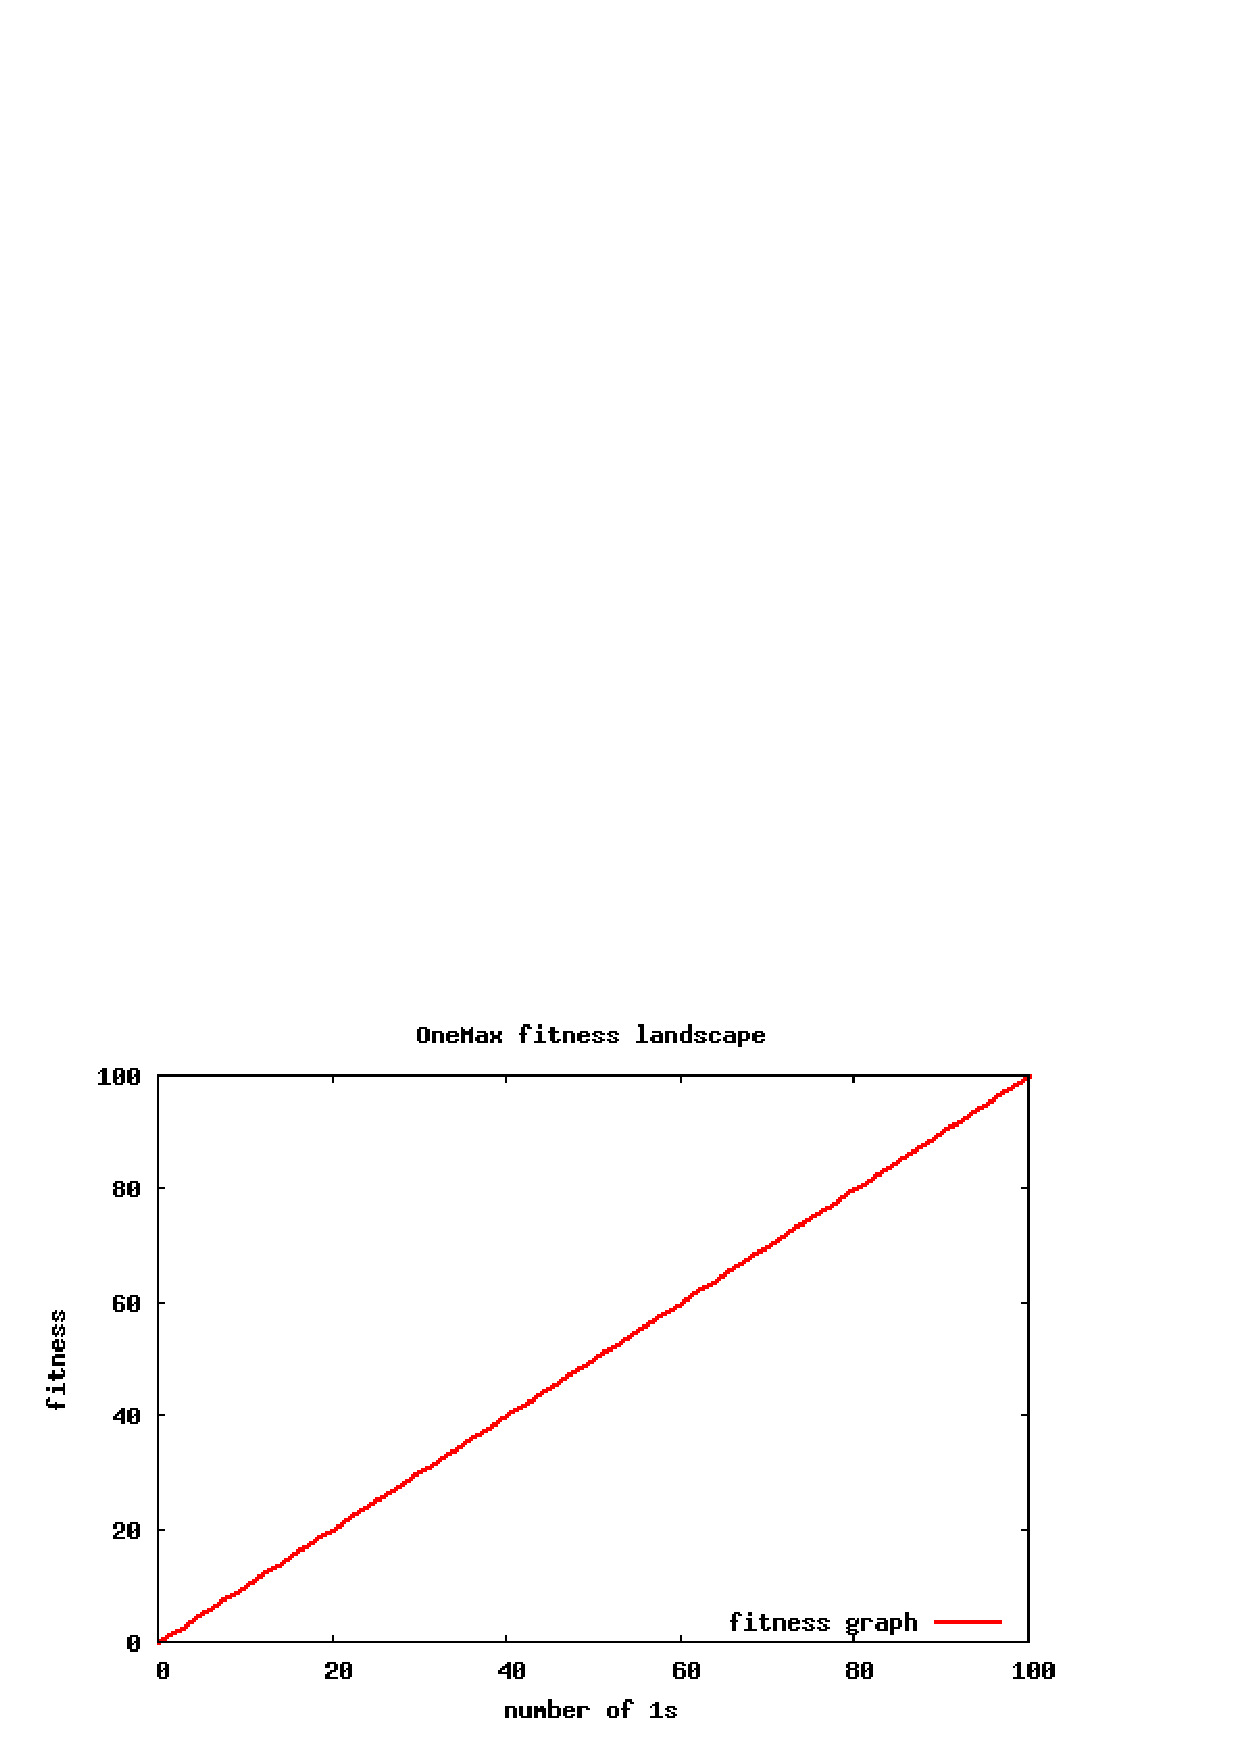
\includegraphics[scale=0.4]{graphs/graph_onemax_fitness_landscape.png}
\mycaption{Fitness Landscape of OneMax}
\label{fitness_landscape_onemax}
\end{wrapfigure}
In this test we examine the behaviour of the algorithms in terms of their {\emph fitness} with varying parameters with the problem OneMax. The goal is to find the string '111\dots', each '1' in a component of an individual gets rewarded by one fitness point. This is also the the main difference to a flat fitness landscape, when selecting individuals for a new generation we do not randomly take \(N\) individuals and calculate our distribution vector \(p\) but we sort all individuals by their fitness and only select the top 50\%.\\
 While the OneMax problem does not represent a problem with a real flat fitness landscape (thus the theory we discussed earlier does not apply here), a local flat fitness landscape can occur if the variance drops and/or the fitness values of the population are very similar (e.g. 010, 100, 001).\\
In our test the problem size ranges from 100 to 500 depending on the convergence speed of the functions that we will examine.\\


%\subsection{Plateau Problem}
%It is basically a OneMax problem with the difference that in a solution three neighbouring bits have to be '1' in order to get one fitness point. E.g. 100.110 would give 0 fitness points while 111.110 or 000.111 would give 1 fitness point. The problem size is of course a multiple of 3, usually 300.
%\begin{figure}[H]
%\includegraphics[scale=0.35]{graph_plateau000_fitness.png}
%\mycaption{Fitness landscape of OneMax with two peaks}
%\label{fitness_landscape_onemax2}
%\end{figure}
%\begin{figure}[H]
%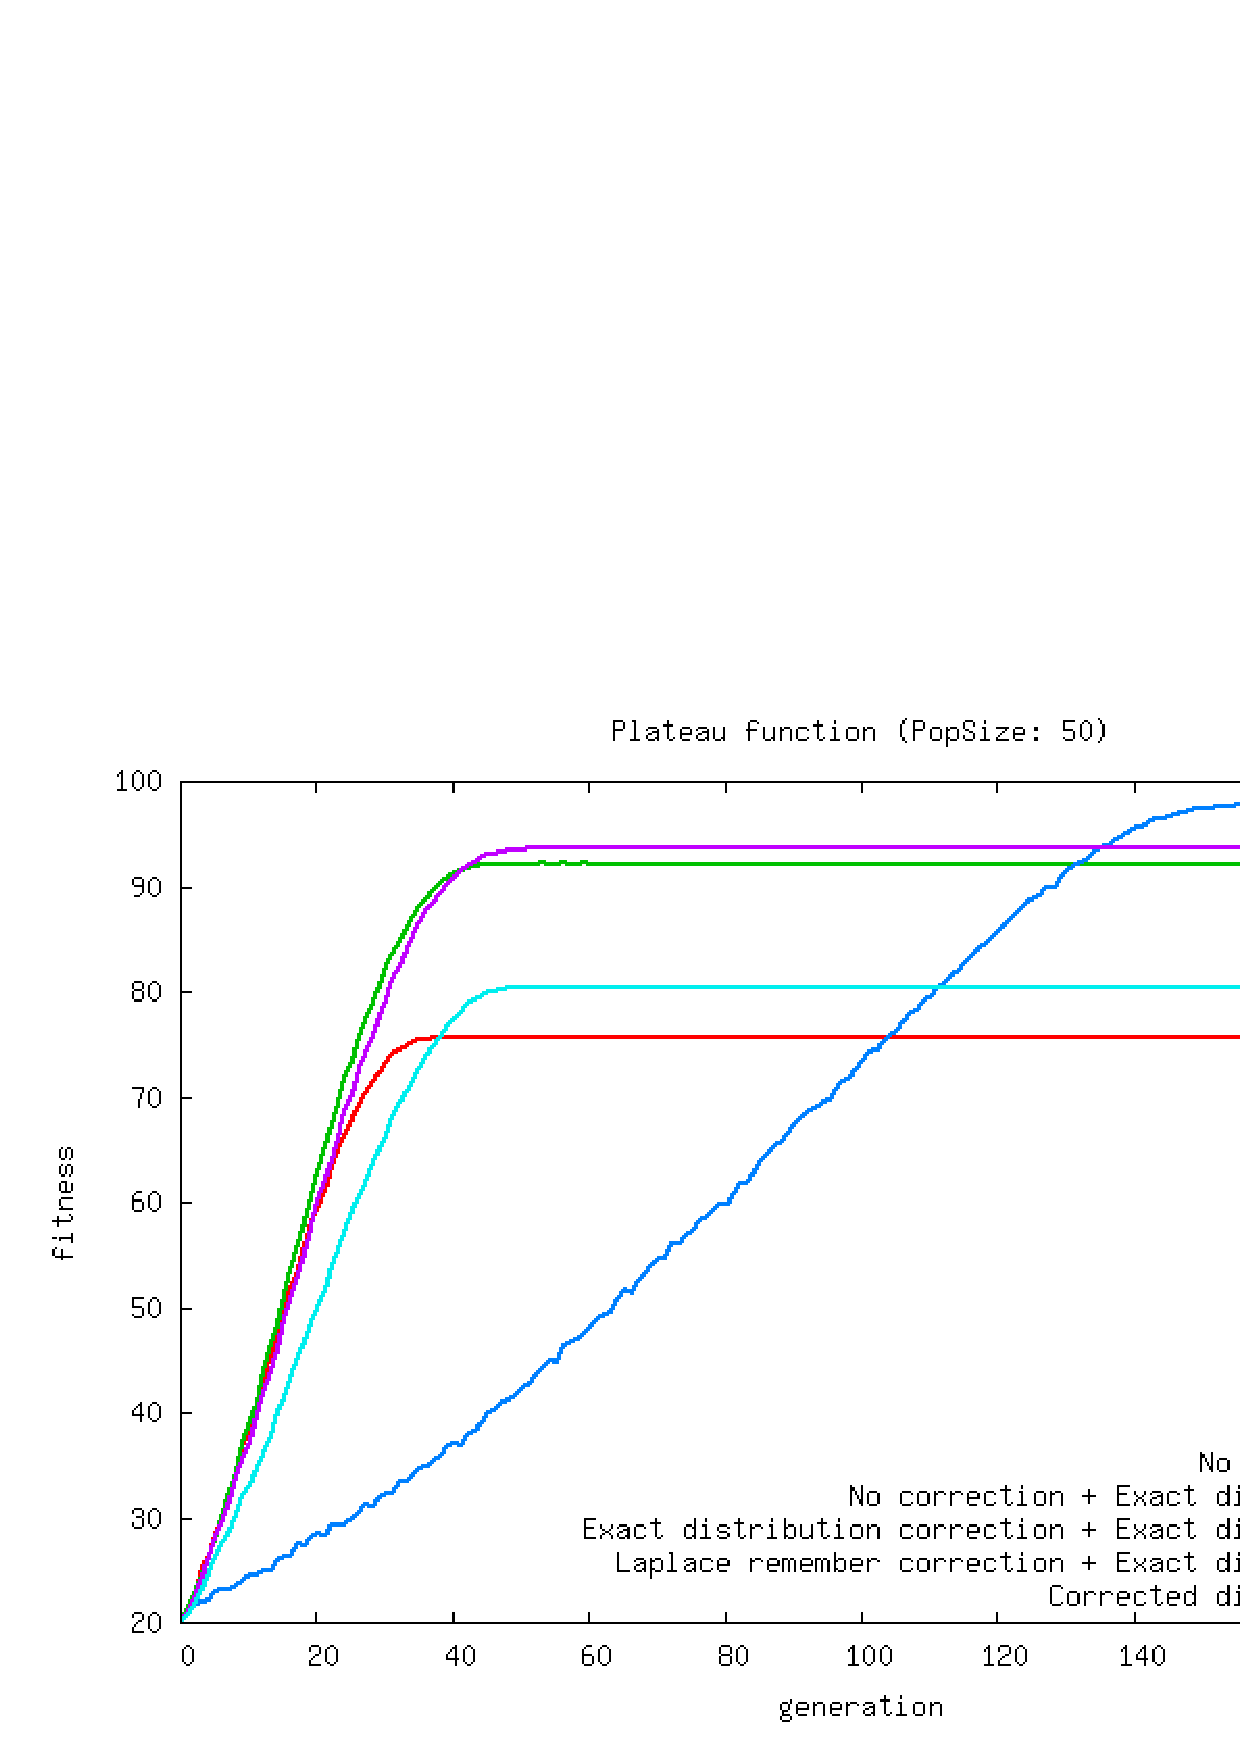
\includegraphics[scale=0.35]{graph_plateau001_fitness.png}
%\mycaption{Fitness landscape of OneMax with two peaks}
%\label{fitness_landscape_onemax2}
%\end{figure}
% TODO
%Remember Laplace Exact Distribution does usually good for small populations and Exact Distribution + Exact Correction has again a low convergence rate but the best fitness with larger populations.

%\newpage
%TODO evtl wieder raus
%\subsection{TwoPeak problem}
%\begin{wrapfigure}{r}[0cm]{6.5cm}
%\vspace{-0.7in}
%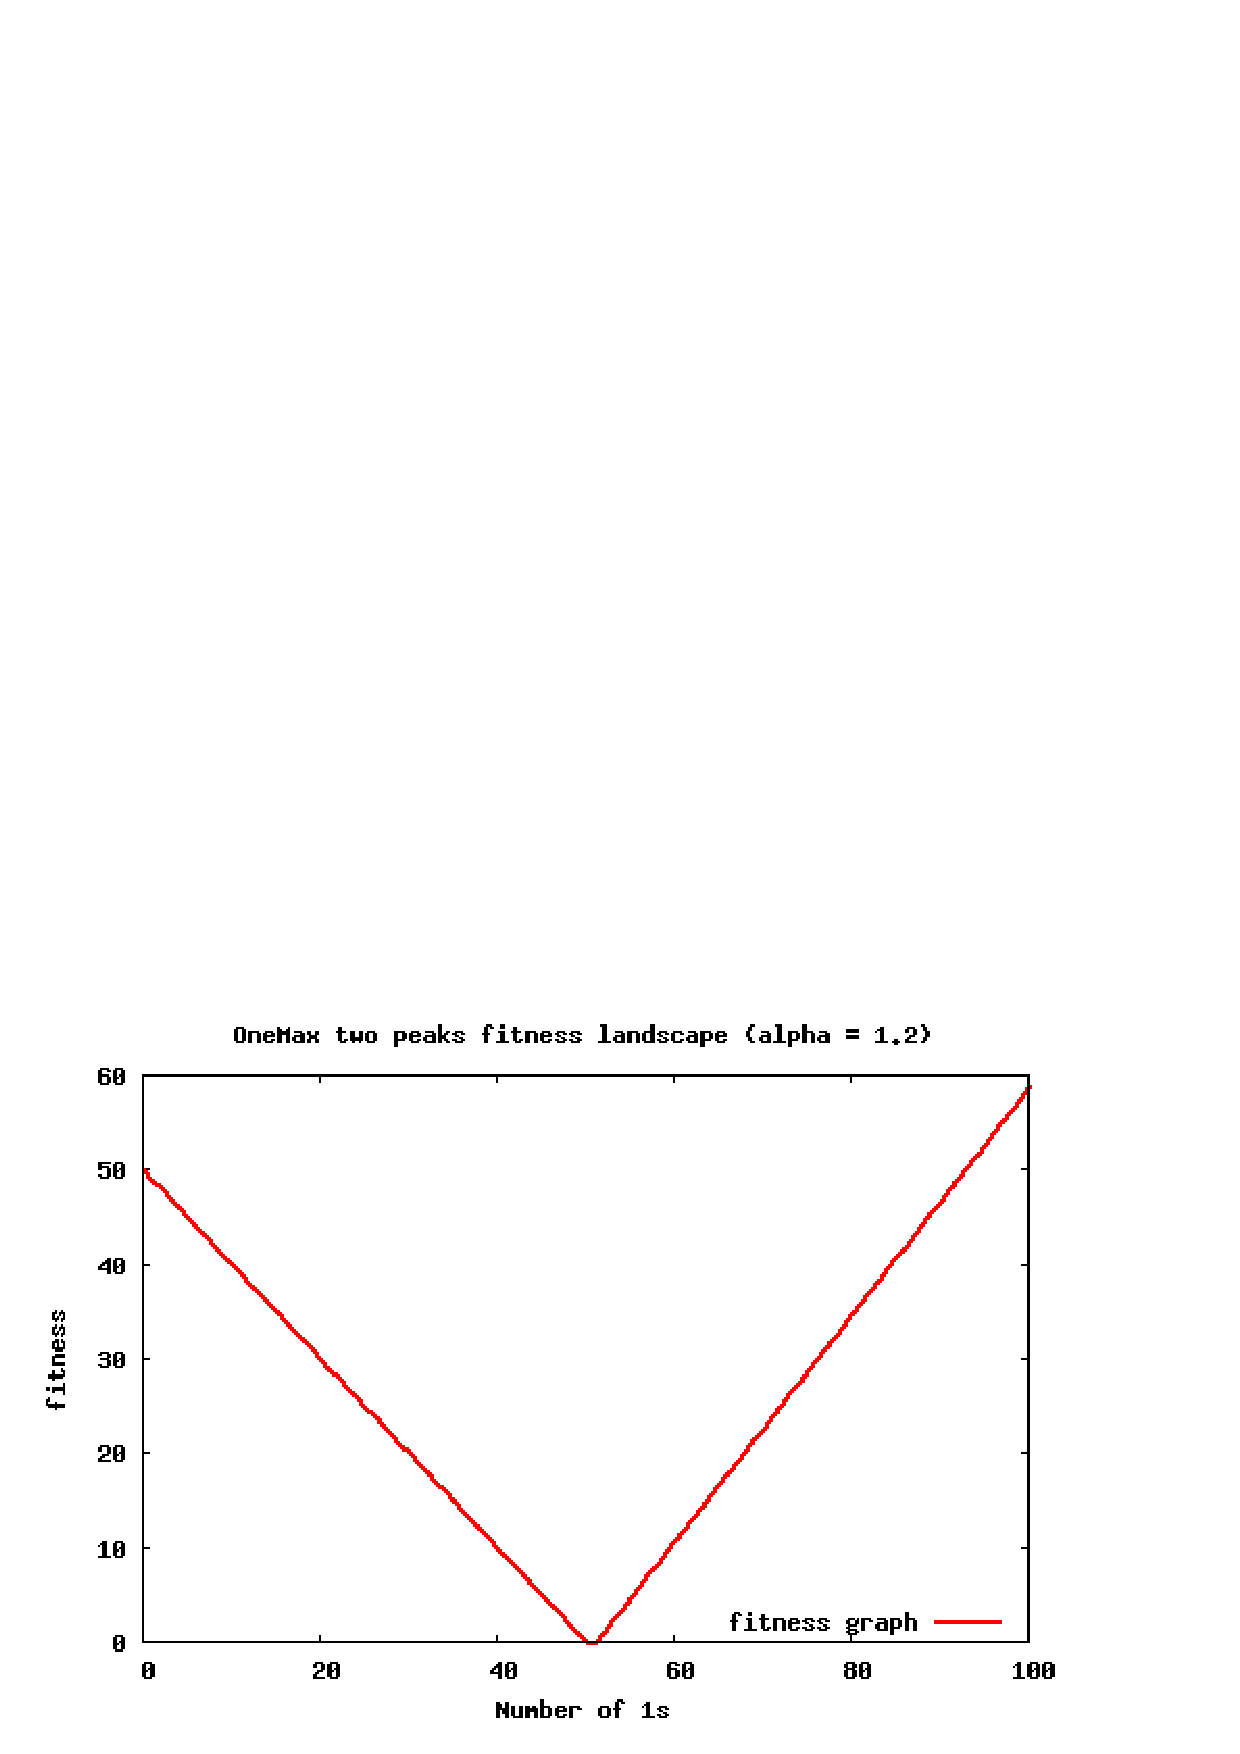
\includegraphics[scale=0.4]{graphs/graph_onemax2_fitness_landscape.png}
%\mycaption{Fitness landscape of TwoPeak}
%\label{twopeak_fitness_landscape_onemax2}
%\end{wrapfigure}

%Similar to the OneMax problem we do count the number of equal values but not only '1's but '0's, too. There are two parameters, one defines the center where we switch from counting '0's to counting '1's and one is a factor which determines how much more (or less) worth is a '1' compared to a '0'.


%%6 different algorithms were tested: ?? TODO


\subsection{Leading-1s problem}

In the Leading-1s problem the fitness is calculated by counting the number of leading '1's. This implies that contrary to OneMax the bit-position is important and the bits are connected, i.e. component \(i\)'s fitness depends on all components \(j\) with \(0 < j < i\). This is more difficult to handle for UMDA's discussed in this report.\\
For this problem keeping correct solutions on lower bit-positions is very important, i.e. lower bit-positions contribute to the total fitness more than higher bit-positions. Any algorithm that keeps up a high diversity in positions that already have the correct value will have a significantly lower fitness.

\subsection{NK Landscape}

From \cite{NKLandscape}:

,,An NK landscape is a real-valued function defined on the set of binary \(n\)-tuples, \(\{0,1\}^{n}\), which is of the form

\begin{equation}
f (x_1, x_2, \dots, x_n) = \sum_{i=1}^{n} f_{i} (x_i, \prod (x_i))
\end{equation}

It is a summation of local fitness functions \(f_{i}\)'s, where each \(f_{i}\) depends on its main variable \(x_{i}\) and the variables in the neighborhood of \(x_{i}\). Here the neighborhood \(\prod (x_{i})\) is a subset of the set \(\{x_{1}, x_{2}, \dots, x_{n}\} \backslash \{x_{i}\}\) and its size \(|\prod_{k}(x_{i})|\) is \(k\). There are two ways to choose the variables in the neighborhood \(\prod (x_{i})\), adjacent neighborhood and random neighborhood. In the NK models with adjacent neighborhood, \(\prod(x_{i})\) consists of the closest \(k\) variables (with a certain to-break) to the main variable \(x_{i}\) with respect to the indices modulo \(n\). In the NK models with random neighborhood, \(\prod(x_{i})\) is composed of the \(k\) variables chosen uniformly at random from \(\{x_{1}, x_{2}, \dots, x_{n}\} \backslash \{x_{i}\}\). Local fitness functions are constructed independently of each other. For each local fitness function, a random value from a probability distribution is assigned for each input.''\\

We will use a similar implementation as \cite{MitchelPotter}, with 'Random(\(x\))' denoting a function that maps \(x\) to a random value. 
\[
f_{i} = \frac{\mbox{Random}(2^{k})}{2^{k}}
\]

That means that wwo function calls with the same parameter (i.e. the same bit pattern) will result in the same value. If a new individual is created with the same pattern it gets the same fitness for this pattern. For \(k = 1\) we would get a similar function as OneMax as there are only two possible values for \(f_{i}\), i.e. we are counting '1's (or '0's). For large values of \(k\) this means that a large portion of memory is needed at the beginning (\(2^{k}\) e.g. 4 GB for \(k = 32\)) so for the implementation we will use a hashtable and relative small numbers (\(k = 10\) and \(n = 50\)).

%\subsection{Knapsack problem}

%This problem is about putting variable number of objects of variable size in a 'rucksack'. The more size of the rucksack is used the higher is the fitness. If the total size of the objects is greater than the size of the rucksack the fitness is zero.
%The main issue with UMDA is how to represent the selection of objects with a binary string. I will use the implementation of \cite{Knapsack}:
%TODO

\newpage
\section{Additional methods}

\subsection{Boundary Correction (BC)}
\begin{wrapfigure}{r}[0cm]{5.5cm}
\vspace{-0.7in}
\includegraphics[scale=0.4]{graphs/graph_correction/graph_random_distribution_boundary_correction.png}
\mycaption{Correction graph for Boundary Correction}
\label{bd_correction_1}
\end{wrapfigure}

An optional correction method is called {\bf Boundary Correction}. It can be used in connection with NoC, RDC and EDC and checks the boundaries of the final value of the distribution vector \(p\). In the case \(p\) gets above \(1 - \beta\) or below \(\beta\) it is corrected to these boundaries:

\[
p = \left\{
\begin{array}{l l}
\beta & \quad \mbox{for \(p < \beta\)}\\
1 - \beta & \quad \mbox{for \(p > 1 - \beta\)}\\
p & \quad \mbox{else}\\
\end{array}
\right.
\]

\subsection{Laplace Correction (LC)}	

\begin{wrapfigure}{r}[0cm]{5.5cm}
\vspace{-0.7in}
\includegraphics[scale=0.4]{graphs/graph_correction/graph_laplace_correction.png}
\mycaption{Correction graph for Laplace Correction}
\label{lc_correction_1}
\end{wrapfigure}

Laplace correction is (so far) more or less the standard in connection with UMDA \cite{LaplaceStandard}. It biases the resulting \(p\) towards \(\frac{1}{2}\) and ensures that components do not get stuck at \(p = 1.0\) or \(p = 0.0\). Basicly it behaves very much like Boundary Correction except that it cannot be combined with another correction method. The general formula for Laplace correction for a component \(i\) is to divide the number of '1's in the selected population plus \(\alpha\) by the size of the selected population plus \(2\alpha\).
\begin{equation}
p_{i} = \frac{k_{i} + \alpha}{N + 2\alpha}
\end{equation}


\subsection{Laplace Remember Correction (LRC)}

\begin{wrapfigure}{r}[0cm]{5.5cm}
\vspace{-0.7in}
\includegraphics[scale=0.4]{graphs/graph_correction/graph_laplace_remember_correction.png}
\mycaption{Correction graph for Laplace Remember Correction with \(p_{t} = 0.25\)}
\label{lrc_correction_1}
\end{wrapfigure}

Another option is to include the distribution vector of the previous generation. We will replace \(\alpha\) in the numerator with \(\tilde{\alpha} = 2 p_{t;i} \alpha\) where \(p_{t+1}\) denotes the new and \(p_{t}\) denotes the old distribution vector. In Figure \ref{lrc_correction_1} you can see that the function changes the new \(p\) to a lower value if the \(p_{t}\) was lower than \(0.5\). Effectively this means that we soften sudden changes between two generations by a small degree.
\[
p_{t+1;i} = \frac{k_{i} + 2 \alpha p_{t;i}}{N + 2 \alpha}
\]

While including previous generations into the generation is not the scope of this report, it is certainly worth further examination. For example we can combine EDC with LRC by first executing EDC and then LRC. See the next chapter for a more detailed analysis.

\newpage
\section{General test configuration}

\subsection{Graph drawing}

The graphs were created with the help of gnuplot 4.0 and g++ 4.0 (gnu C++), the actual program is available on CD-ROM. 50 separate runs were made for each parameter setting and algorithm because all algorithms are based on random numbers. In addition each run consists of a number of generations. In each generation the best fitness value that was found so far in that run is recorded. Then for each generations all recorded values are averaged between the runs and drawn as a graph. I.e. if we have one run (1 1 2 5 5 8) and another run (2 2 2 3 3 5) then our resulting graph would be (1.5 1.5 2 4 4 6.5).

\subsection{Population size}

Depending on the problem type, problem size and algorithm different population sizes ranging from 10 to 100 were tested. Also for each single configuration several different population sizes were tested because the convergence speed differ between the methods. Larger populations automatically result in more diversity and less diversity loss in each generation.

\subsection{Selection size N}

For problem types that do not use a flat fitness landscape we are interested in their fitness. We usually select the top 50\% from the population in order to calculate the distribution vector \(p\). Higher selection rates will reduce the convergence speed because we are including below average solutions in \(p\) while lower selection rates will significantly increase the diversity loss. If the convergence speed is reduced the method will have difficulties to reach or maintain good solutions either because the diversity dropped already to zero or (with Boundary Check or Laplace Correction, see next chapter for a definition) the high diversity holds back good solutions from spreading through the population. It is not the scope of this report to discuss this subject in detail but to present the general effect of different selection sizes.\\

%pop10 und pop30
\begin{figure}[H]
\hspace{-0.5in}
\includegraphics[scale=0.5]{graphs/graph_nk1163198367/graph_nk000_fitness.png}
\includegraphics[scale=0.5]{graphs/graph_nk1163198367/graph_nk001_fitness.png}
\mycaption{Different selection sizes without boundary correction, NK-Landscape, Population size 10 and 30}
\label{selectionsize2}
\end{figure}

In Figure \ref{selectionsize1} we can clearly see the trade-off between speed and quality and that elitism (i.e. small selection size) with methods that do not prevent uniformity in the population (i.e. no Boundary Correction or Laplace Correction) is very bad. We can see this also with more difficult problems like the NK landscape (Figure \ref{selectionsize2}), any extreme value for selection size generally does not improve the search.


%TODO
%\begin{figure}[H]
%\hspace{-0.5in}
%\includegraphics[scale=0.5]{graphs/graph_leading1162405415/graph_leading000_fitness.png}
%\includegraphics[scale=0.5]{graphs/graph_onemax1162405710/graph_onemax000_fitness.png}
%\mycaption{Different selection sizes without boundary correction}
%\label{selectionsize1}
%\end{figure}

On the other hand, with Boundary Correction, we can see in Figure \ref{selectionsize3} that elitism clearly pays off (primarily in speed) with easier problems like LeadingOnes while being below average with more difficult problems like the NK landscape. So we can conclude that generally a selection size of 50\% is a good standard value.

%pop10 pop30
\begin{figure}[H]
\hspace{-0.5in}
\includegraphics[scale=0.5]{graphs/graph_nk1163198192/graph_nk000_fitness.png}
\includegraphics[scale=0.5]{graphs/graph_nk1163198192/graph_nk001_fitness.png}
\mycaption{Different selection sizes with boundary correction, NK-Landscape, Population size 10 and 30}
\label{selectionsize3}
\end{figure}

%pop30 und pop30
\begin{figure}[H]
\hspace{-0.5in}
\includegraphics[scale=0.5]{graphs/graph_leading1163208885/graph_leading001_fitness.png}
\includegraphics[scale=0.5]{graphs/graph_leading1163209153/graph_leading001_fitness.png}
\mycaption{Different selection sizes with boundary correction, LeadingOnes, Population size 10 and 30}
\label{selectionsize3}
\end{figure}

\newpage
\section{Discussion and Comparison between the correction methods}

\subsection{Boundary Correction}

\begin{wrapfigure}{r}[0cm]{5.5cm}
\vspace{-0.7in}
\includegraphics[scale=0.4]{graphs/graph_flat1163209833/graph_flat000_diversity.png}
\mycaption{With boundary correction the diversity is held at a certain level (Flat fitness landscape)}
\label{bd_correction_2}
\end{wrapfigure}

You can see in Figure \ref{bd_correction_2} that with BC the diversity is held at a certain level. For each component there is always at least a chance of \(\beta\) to switch between '0' and '1'. On the one side this has the positive effect that theoretically a better or even the optimal solution will be found. On the other hand single components that already contain an optimal value can switch back to the wrong value.\\

If \(\beta\) is too large the function will have problems preserving the solution, if \(\beta\) is too low the function might need much more time to get out of a local optimum. For example in the case of an OneMax problem to get from 99 '1's to 100 '1's we not only need to generate another '1' but we have to preserve all the other 99 '1's, too. Thus we can conclude that a good value for \(\beta\) is dependent on all parameters, the population size, the problem type, the correction type and especially the problem size. In addition we can conclude that a very low value (relative to the problem size) for \(\beta\) will always be positive in the long run while reducing its convergence speed a little. In Figure \ref{bd_correction_3} you can see that there values for \(\beta\) with which EDC+BC clearly is better than EDC without BC (i.e. \(\beta = 0\)) and that the optimal value depends on the population size.

\begin{figure}[H]
\hspace{-0.5in}
\includegraphics[scale=0.5]{graphs/graph_onemax1163211796/graph_onemax000_fitness.png}
\includegraphics[scale=0.5]{graphs/graph_onemax1163211796/graph_onemax000_diversity.png}
\mycaption{Different values for \(\beta\), OneMax}
\label{bd_correction_3}
\end{figure}

\begin{figure}[H]
\hspace{-0.5in}
\includegraphics[scale=0.5]{graphs/graph_nk1163212098/graph_nk000_fitness.png}
\includegraphics[scale=0.5]{graphs/graph_nk1163212098/graph_nk001_fitness.png}
\mycaption{Different values for \(\beta\), NK-Landscape, Population size 10 and 30}
\label{bd_correction_4}
\end{figure}

When combining Boundary Correction with either RDC or EDC we will face the same problem as discussed with Exact Distribution. When we change our \(p\) before we create our population we will also have to adapt the Correction methods themselves. This could be a small source of error and probably have to be researched more closely if there is an algorithm that performs better than RDC+BC or EDC+BC by including \(\beta\) in its calculation.

\subsection{Laplace Correction}

Again the optimal value for \(\alpha\) depends on the type of the problem and the problem parameters. While we have approximately \(\alpha = 0.03\) as the optimal value for the OneMax problem we have approximately \(\alpha = 0.15\) as the optimal value with the Plateau problem in Figure \ref{laplace_alpha_1} and the NK problem in Figure \ref{laplace_alpha_2}. In addition there is always the trade-off between convergence speed and fitness for some problems. If we set \(\alpha\) very low we have a chance to get out of uniformity of a component but a low convergence speed. If we use higher values for \(\alpha\) we get faster to the optimal solution but are no longer able to keep good solutions.

%pop30
\begin{figure}[H]
\hspace{-0.5in}
\includegraphics[scale=0.5]{graphs/graph_nk1163212946/graph_nk000_fitness.png}
\includegraphics[scale=0.5]{graphs/graph_leading1163214649/graph_leading000_fitness.png}
\mycaption{\(\alpha\) influences the effectiveness of Laplace correction but is problem-dependent, NK-Landscape and LeadingOnes}
\label{laplace_alpha_1}
\end{figure}


%TODO evtl raus
%\begin{figure}[H]
%\hspace{-0.5in}
%\includegraphics[scale=0.5]{graphs/graph_nk1162146485/graph_nk000_fitness.png}
%\includegraphics[scale=0.5]{graphs/graph_leading1162147298/graph_leading000_fitness.png}
%\mycaption{\(\alpha\) influences the effectiveness of Laplace correction but is problem-dependent}
%\label{laplace_alpha_2}
%\end{figure}


%TODO Vergleiche innerhalb von Gruppen, also No correction No correction+bounded, diversity correction mit diversity correction+bounded etc.

%\begin{figure}[H]
%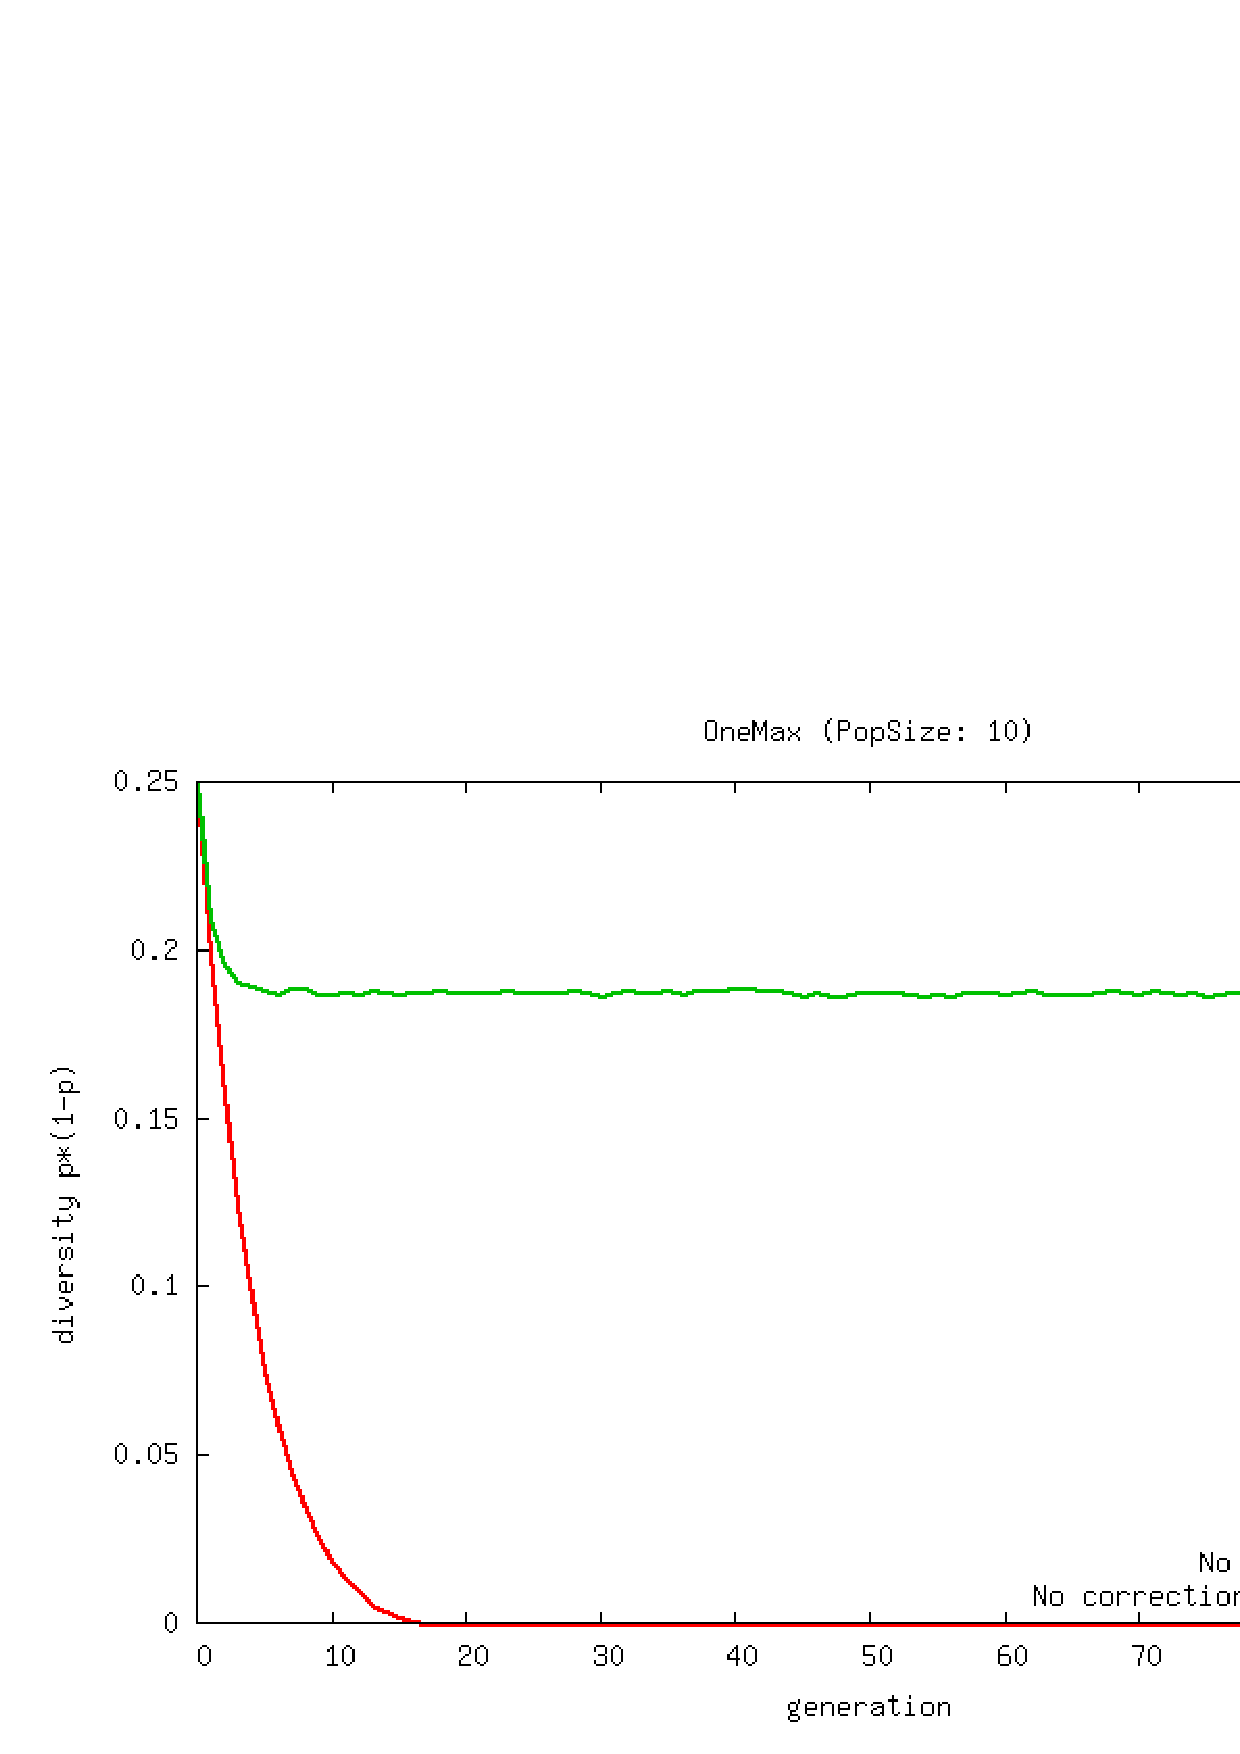
\includegraphics[scale=0.35]{graph_onemax_no_correction_bounded_diversity0.png}
%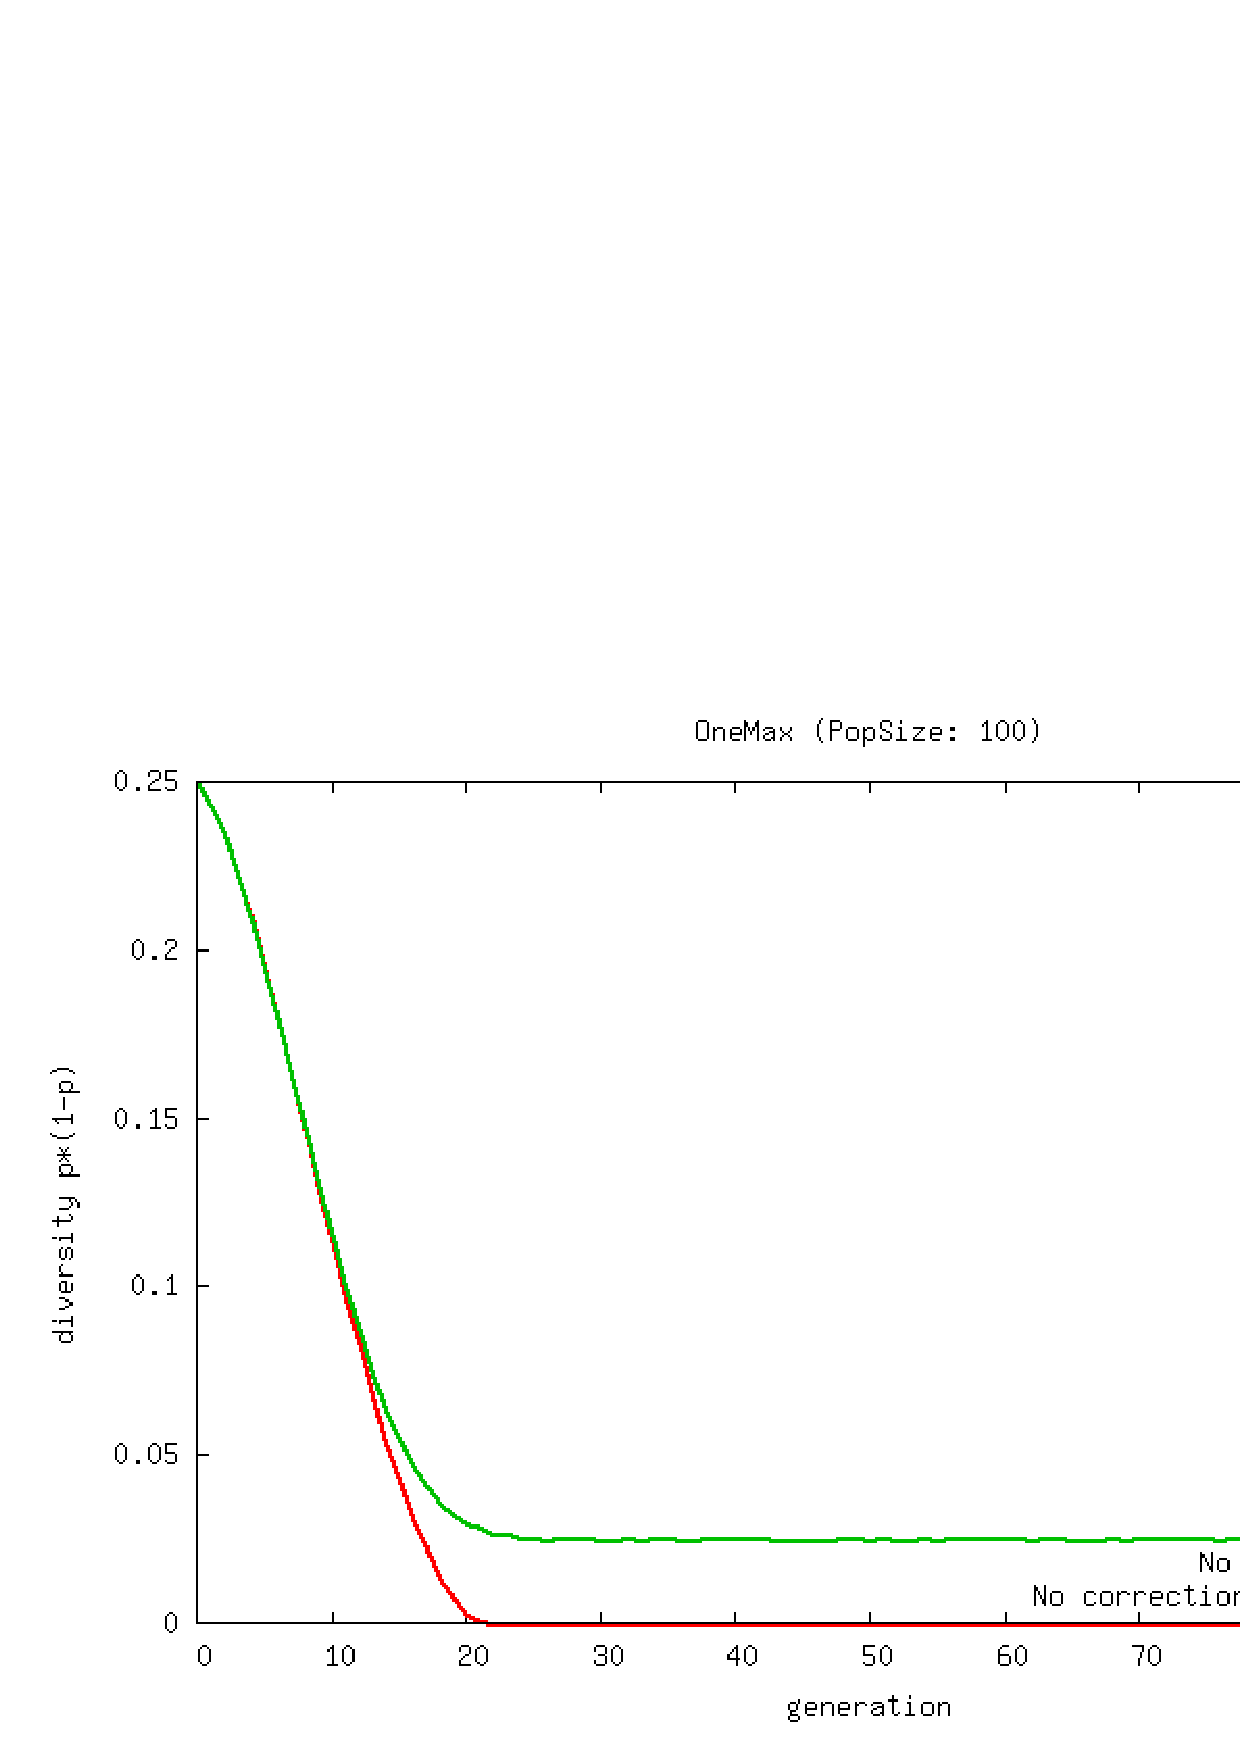
\includegraphics[scale=0.35]{graph_onemax_no_correction_bounded_diversity1.png}
%\mycaption{With boundary check the diversity is held at a constant level}
%\label{bounded_1}
%\end{figure}
%TODO 


%For onemax we clearly see that these two opposite effects let the function converge at a lower level:

%TODO While it has a chance to find a better solution (in contrary to the method without correction) it has trouble keeping up the correct values that were found so far.

%TODO With higher population sizes this effect vanishes as \(\frac{1}{M}\) becomes smaller.

%\begin{figure}[H]
%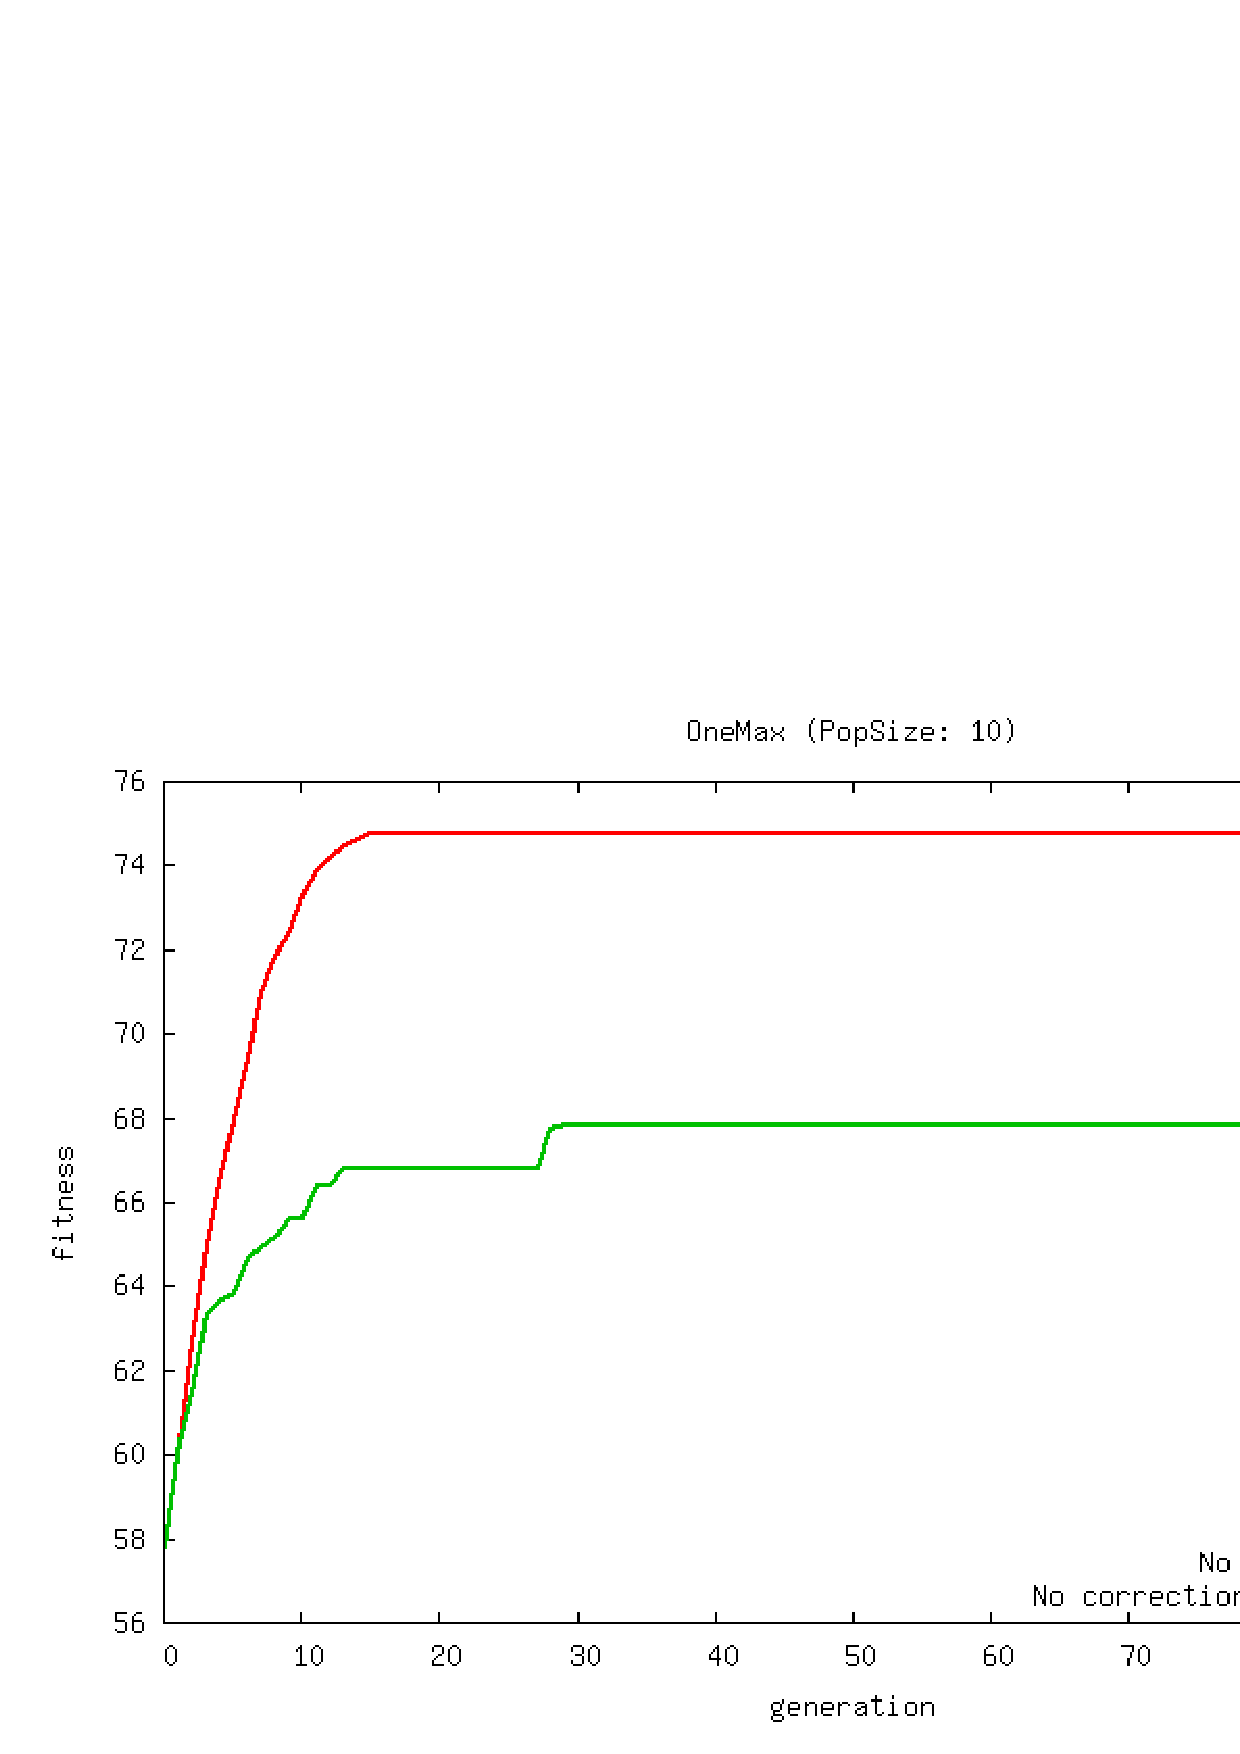
\includegraphics[scale=0.35]{graph_onemax_no_correction_bounded_fitness0.png}
%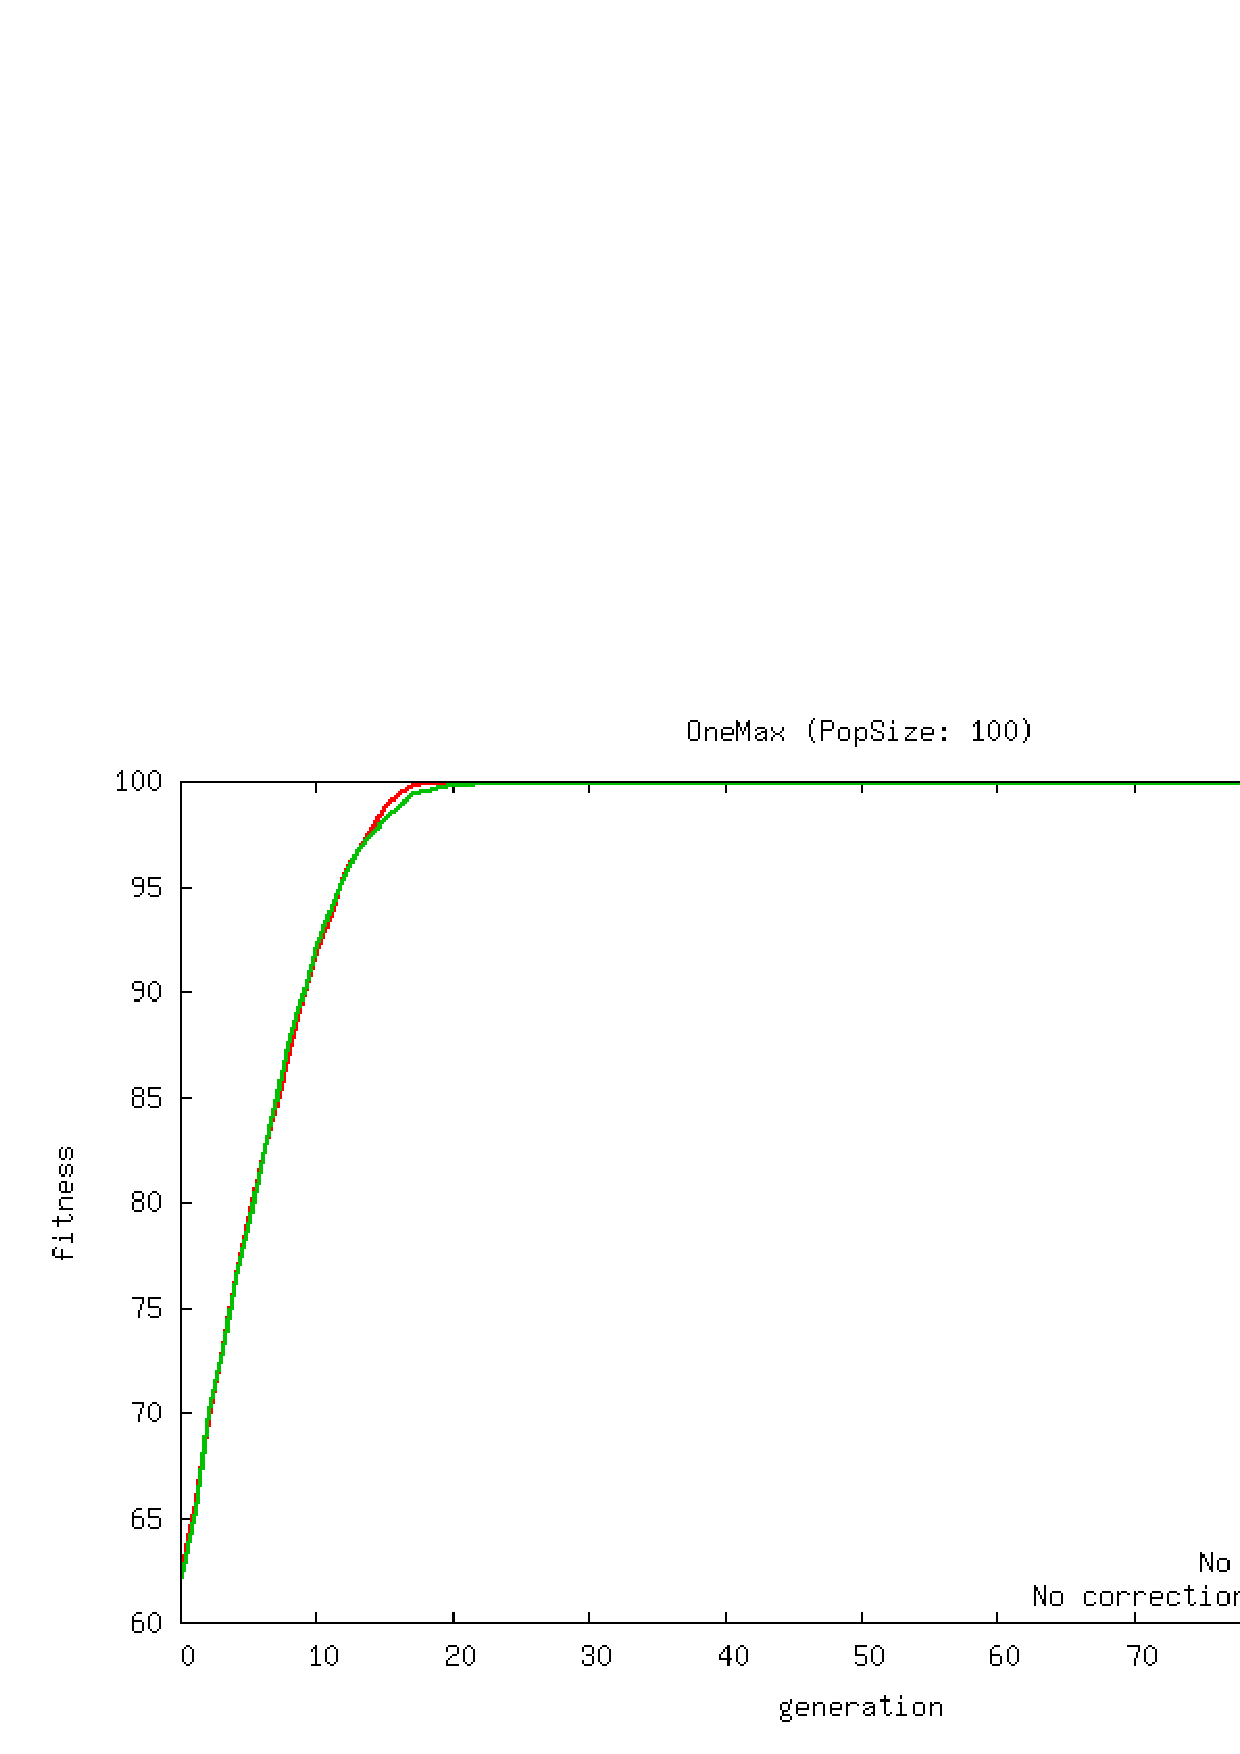
\includegraphics[scale=0.35]{graph_onemax_no_correction_bounded_fitness1.png}
%\mycaption{With boundary check the diversity is held at a constant level}
%\label{bounded_2}
%\end{figure}

%\begin{figure}[H]
%\hspace{-0.5in}
%\includegraphics[scale=0.5]{graphs/graph_onemax1161008942/graph_onemax000_diversity.png}
%\includegraphics[scale=0.5]{graphs/graph_onemax1161008942/graph_onemax000_diversity.png}
%\mycaption{TEST}
%\label{bounded_3}
%\end{figure}

%------------ TODO END


\subsection{Boundary vs. Laplace Correction}

As we have discussed in the previous chapter, both Laplace Correction and Boundary Correction does prevent \(p\) from getting near the boundary values \(p = 0.0\) and \(p = 1.0\). In addition LC biases the resulting \(p\) to \(\frac{1}{2}\) due to the lower gradient. We can expect that Laplace Correction outperforms a simple Boundary Correction in terms of variance on a flat fitness landscape, the question is if this bias is significant.\\
For the test we will look at configurations of \(\alpha\) and \(\beta\) that change \(p\) at the borders to the same values. Laplace Correction corrects \(p = 0\) to \(\frac{\alpha}{N + 2\alpha}\), Boundary Check corrects \(p = 0\) to \(\beta\), so in order to compare the behaviour at the borders we set \(\beta = \frac{\alpha}{N + 2\alpha}\). In Figure \ref{boundedvslaplace1} we have set \(\alpha = 0.1\) and \(beta = 0.0193\) (for N = 5). As expected LC provides more variance but as we can see in the fitness graph at the cost of a lower convergence speed. 

\begin{figure}[H]
\hspace{-0.5in}
\includegraphics[scale=0.5]{graphs/graph_onemax1163347837/graph_onemax000_diversity.png}
\includegraphics[scale=0.5]{graphs/graph_onemax1163347837/graph_onemax000_fitness.png}
\mycaption{Comparison of diversity and fitness, OneMax (Population size 10)}
\label{boundedvslaplace1}
\end{figure}

With a more difficult problem like a NK-landscape we see that LC again keeps up a higher level of diversity which causes it to be slower at the beginning but reaching a higher level of fitness later (Figure~\ref{boundedvslaplace3}).
\begin{figure}[H]
\hspace{-0.5in}
\includegraphics[scale=0.5]{graphs/graph_nk1163349298/graph_nk000_fitness.png}
\includegraphics[scale=0.5]{graphs/graph_nk1163349298/graph_nk000_diversity.png}
\mycaption{Comparison of fitness and diversity, NK-Landscape (Population size 10)}
\label{boundedvslaplace3}
\end{figure}

In conclusion we can say that using Laplace Correction is not much different than Boundary Correction. Due to the lower gradient of the correction function it has a lower convergence rate which allows the method to search a longer in a population with higher diversity at the beginning. The main disadvantage of LC is that we can not easily combine it with other correction functions. Boundary Correction on the other hand only changes the borders of the correction function and will be used in this paper in connection with all other methods.

\subsection{Laplace Remember Correction}

Tests have shown that the value for \(\alpha\) is not significant (see Figure \ref{laplace_remember_alpha_1}) so we set \(\alpha = 1.0\). As the method does not prevent extreme values for \(p\) we will also use a Boundary Correction in connection with LRC. 

\begin{figure}[H]
\hspace{-0.5in}
\includegraphics[scale=0.5]{graphs/graph_flat1163339386/graph_flat000_diversity.png}
\includegraphics[scale=0.5]{graphs/graph_onemax1163339355/graph_onemax000_fitness.png}
\mycaption{No significant difference between different values of \(\alpha\) (Flat fitness landscape, OneMax) in diversity loss and fitness}
\label{laplace_remember_alpha_1}
\end{figure}

LRC behaves similarly as the underlying distribution function as can seen in Figure \ref{laplace_remember_2}. Thus LRC alone does not give have any real advantage but we section we will try to combine LRC with EDC.

\begin{figure}[H]
\hspace{-0.5in}
\includegraphics[scale=0.5]{graphs/graph_leading1163345629/graph_leading000_fitness.png}
\includegraphics[scale=0.5]{graphs/graph_nk1163345894/graph_nk000_fitness.png}
\mycaption{Similar behavior of LRC as the underlying distribution method (Leading Ones and NK-Landscape, population size 10)}
\label{laplace_remember_2}
\end{figure}


\subsection{EDC with Laplace Remember Correction}

As stated earlier we can combine EDC with LRC by first executing EDC and then LRC with the parameters \(p_{t;i}\) and \(k_{i} = q_{i} \cdot N\), with \(q_{i}\) being the distribution vector corrected by EDC. Preventing sudden changes might be useful in connection with the Distribution Correction because the correction graph (Figure \ref{dc_correction_1}) has a large gradient left of \(p_{1}\) and right of \(p_{2}\). 

\begin{figure}[H]
\hspace{-0.5in}
\includegraphics[scale=0.5]{graphs/graph_flat1163359845/graph_flat000_diversity.png}
\includegraphics[scale=0.5]{graphs/graph_onemax1163359950/graph_onemax00_fitness.png}
\mycaption{Comparison between EDC+LRC and EDC in terms of their diversity and fitness (Flat fitness landscape and Onemax, Population size 30)}
\label{laplace_remember_edc_1}
\end{figure}

While some runs show a better fitness by a small margin, others do not.

\begin{figure}[H]
\hspace{-0.5in}
\includegraphics[scale=0.5]{graphs/graph_flat1163359845/graph_flat000_diversity.png}
\includegraphics[scale=0.5]{graphs/graph_onemax1163359950/graph_onemax00_fitness.png}
\mycaption{Comparison between EDC+LRC and EDC in terms of their diversity and fitness (Flat fitness landscape and Onemax, Population size 30)}
\label{laplace_remember_edc_1}
\end{figure}

The original idea was that we prevent sudden changes by including the old distribution vector. If we not just use the Laplace Correction approach but directly average (EDC+AV+BC) between the old and the current distribution vector we do get an even slower convergence rate and again with a higher maximum fitness level. In conclusion we can say that ED+BC, EDC+BC and EDC+AV+BC provide the best fitness speed trade-off



\newpage



%\subsection{Corrected Distribution vs. Exact Corrected Distribution}

%\begin{figure}[H]
%\includegraphics[scale=0.5]{graphs/graph_onemax1162151659/graph_onemax000_fitness.png}
%\includegraphics[scale=0.5]{graphs/graph_plateau1162152446/graph_plateau000_fitness.png}
%\mycaption{\(\alpha\) influences the effectiveness of Laplace correction but is problem-dependent}
%\label{laplace_alpha_1}
%\end{figure}

%\begin{figure}[H]
%\includegraphics[scale=0.5]{graphs/graph_leading1162142917/graph_leading000_fitness.png}
%\includegraphics[scale=0.5]{graphs/graph_nk1162145639/graph_nk000_fitness.png}
%\mycaption{Comparison of fitness}
%\label{erdvscd1}
%\end{figure}

%\begin{figure}[H]
%\includegraphics[scale=0.5]{graphs/graph_haystack1162144026/graph_haystack000_fitness.png}
%\includegraphics[scale=0.5]{graphs/graph_haystack1162144026/graph_haystack000_diversity.png}
%\mycaption{Comparison of fitness}
%\label{erdvscd2}
%\end{figure}


%Without Boundary Correction we can clearly see in Figure (\ref{erdvscd1}) that EDC is better than ED and RDC is better than RD and EDC is better than RDC:
%\begin{figure}[H]
%\hspace{-0.5in}
%\includegraphics[scale=0.5]{graphs/graph_leading1162416230/graph_leading001_fitness.png}
%\includegraphics[scale=0.5]{graphs/graph_leading1162416230/graph_leading001_diversity.png}
%\mycaption{Comparison of fitness without Boundary Correction}
%\label{erdvscd1}
%\end{figure}

%With Boundary Correction we have to be careful not to set \(\beta\) too high or, in connection with our correction methods, we will get worse results than without distribution correction (Figure \ref{erdvscd2}). This is because with the LeadingOnes problem it is important for lower bit positions to keep their (correct) values.
%\begin{figure}[H]
%\hspace{-0.5in}
%\includegraphics[scale=0.5]{graphs/graph_leading1162414535/graph_leading000_fitness.png}
%\includegraphics[scale=0.5]{graphs/graph_leading1162416727/graph_leading000_fitness.png}
%\mycaption{Comparison of fitness with a small population}
%\label{erdvscd2}
%\end{figure}

%This is also because of the low population size. Looking at a larger population (Figure \ref{erdvscd3}), the difference becomes more clear, although with \(\beta = 0.01\) all four methods converge before they reach the optimum.

%\begin{figure}[H]
%\hspace{-0.5in}
%\includegraphics[scale=0.5]{graphs/graph_leading1162414535/graph_leading001_fitness.png}
%\includegraphics[scale=0.5]{graphs/graph_leading1162416727/graph_leading001_fitness.png}
%\mycaption{Comparison of fitness with a larger population}
%\label{erdvscd3}
%\end{figure}

%With the NK-Landscape it is more important to keep a higher diversity so we can see in Figure \ref{erdvscd4} again a case for Exact Distribution Correction:
%\begin{figure}[H]
%\hspace{-0.5in}
%\includegraphics[scale=0.5]{graphs/graph_nk1162417290/graph_nk000_fitness.png}
%\includegraphics[scale=0.5]{graphs/graph_nk1162417290/graph_nk001_fitness.png}
%\mycaption{Comparison of fitness with a larger population}
%\label{erdvscd4}
%\end{figure}

%\begin{figure}[H]
%\includegraphics[scale=0.4]{graphs/graph_onemax1162144026/graph_onemax000_fitness.png}
%\mycaption{Comparison of fitness}
%\label{erdvscd3}
%\end{figure}

%low population size -> bd
%flat
%onemax

%TODO Beschreibungen und mehr Beispiele

\section{Fields of further research}

There are several open points in this report that were not discussed or left open for further research. Firstly the EDC can be improved by including the rounding error in the calculation. As the distribution vector \(p\) can hold only a limited number of values (\(N+1\) values) prior to the correction it is certainly possible to solve this numerically with a limited accuracy.\\
In addition the complete proof for equation~\ref{eq:dcorrection} is missing and is only demonstrated by Maple to be correct.\\
Also there is missing a rule to determine the optimal values for \(\beta\) in the Boundary Correction method in connection with the parameters (problem size/type and population size). It was demonstrated that the results can be influenced very negatively when choosing too large values for \(\beta\).\\
Another point is that, if applied in a real application, the calculation time maybe another important factor. It was shown that EDC performed better than ED but only by a relatively small margin. EDC needs another calculation step and a table access respectively and needs more generations to reach the (higher) convergence level so it might be slower alltogether.\\
Although it reaches a lower fitness level, LRC in connection with EDC might be the answer concerning the convergence speed and fitness trade-off. It needs more research to determine how to use the distribution vectors of previous generations effectivly.\\
At last other forms of EDAs where a dependency between the components is included in the calculation need to be researched using similar methods of correcting their diversity loss as demonstrated in this report with UMDAs.

\newpage
Ich versichere hiermit wahrheitsgem\"a\"s, die Arbeit bis auf die dem Aufgabensteller bereits bekannte Hilfe selbstst\"andig angefertigt, alle benutzten Hilfsmittel vollst\"andig und genau angegeben und alles kenntlich gemacht zu haben, was aus Arbeiten anderer unver\"andert oder mit Ab\"anderungen entnommen wurde.
\newpage
\begin{thebibliography}{99}
\bibitem{Shapiro} {\sc Shapiro, J.L.:}  \textit{Diversity loss in general estimation of distribution algorithms}, 2006.
\bibitem{Unknown1} {\sc Unkonwn:}  \textit{Source for |A| > 2 handling}.
\bibitem{LaplaceStandard} {\sc Unkonwn:}  \textit{Source for Laplace Standard UMDA}.
\bibitem{Muehlenbein} {\sc H. Muehlenbein and G. Paasz:}  \textit{From recombination of genes to the estimation of distributions: I. binary parameters.}, H.-M. Voigt, W. Ebeling, I. Rechenberg, and H.-P. Schwefel, editors, Parallel Problem Solving from Nature-PPSN IV, pages 178-187, Berlin, 1996. Springer. TODO
\bibitem{NKLandscape} {\sc Y. Gao and J. Culberson:}  \textit{An Analysis of Phase Transition in NK Landscapes}, http://www.cs.cmu.edu/afs/cs/project/jair/pub/volume17/gao02a.ps.Z
\bibitem{MitchelPotter} {\sc Potter, M.A.:}  \textit{NK-landscape problem generator}.
\bibitem{Rucksack} {\sc Unkonwn:}  \textit{Source for Rucksack UMDA representation}.


%http://www.comp.rgu.ac.uk/staff/ss/Publications/GECCO2005.pdf

\end{thebibliography}
\end{document}

